\chapter{脉搏波的预处理与特征参数提取}
\section{引言}
本研究使用的PPG数据来源自自主进行的临床实验,本章从实验设备、实验流程与数据导出等方面对其进行介绍。
利用常用的统计分析方法,对临床实验被试的人口统计学特征进行分析。
介绍PPG的预处理涉及的信号滤波、波形检测、切迹检测、基线漂移处理、信号重采样与数据标准化等过程。
提出一种可应用于多平台、多研究背景的基于初筛—复核—决策的新型PPG波形检测算法。
最后,汇总介绍常见的PPG时域特征参数。

本章研究内容的框架图如\autoref{fig:frameworks3}所示。

\begin{figure}[htbp]
    \centering
    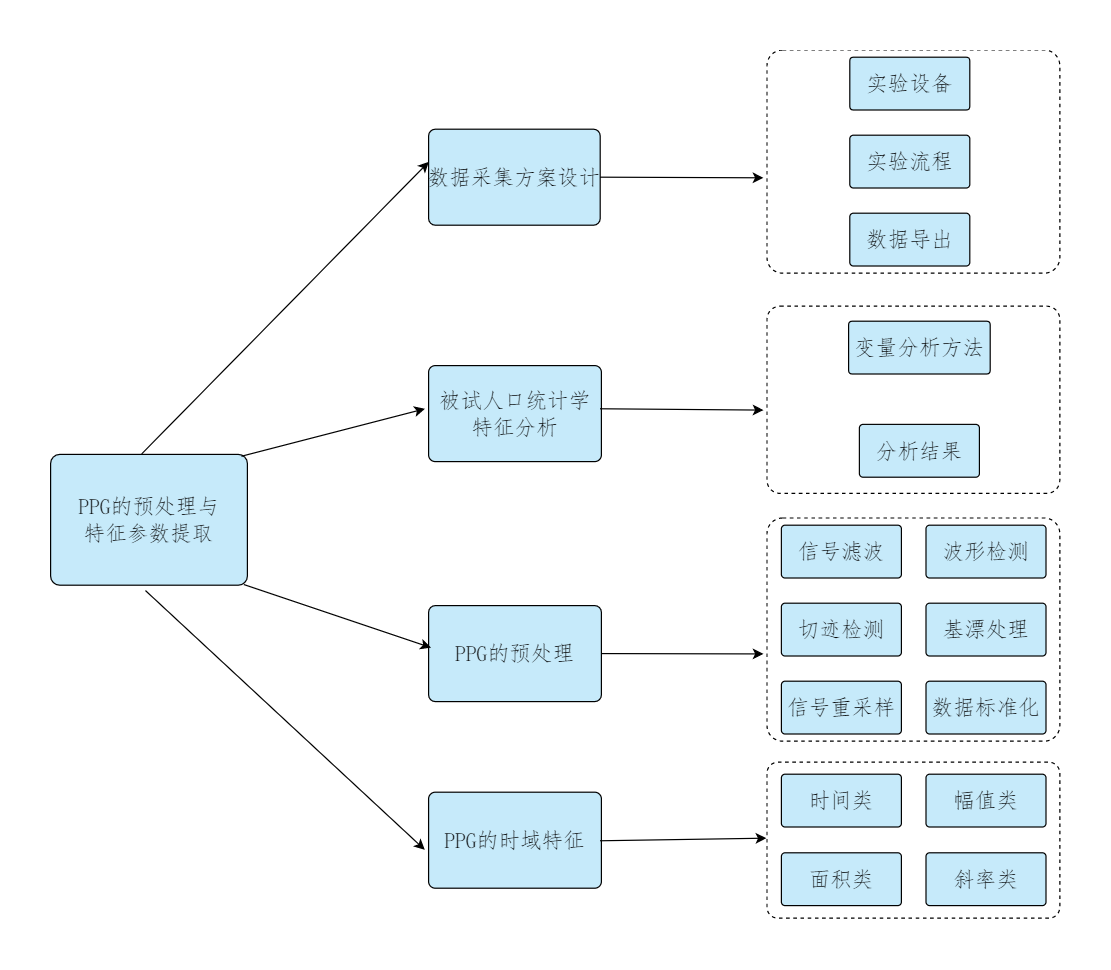
\includegraphics[width=0.85\linewidth]{pulse_preprocess/frameworks3}
    \caption{\label{fig:frameworks3}第三章研究内容框架图}
\end{figure}
\section{临床数据实验}
本研究于2017年6月至2019年4月期间在浙江大学医学院附属妇产科医院进行了临床数据采集实验。
实验通过了浙江大学医学院附属妇产科医院医学伦理委员会的审查(审查编号:20170131),所有被试孕妇均知晓研究目的及具体实验流程,并签署了知情同意书。
其中,实验组为确诊PE的孕妇,对照组为正常妊娠孕妇。
由于实验组孕妇均已确诊PE,不同程度地出现了血压升高等症状,因此实验组孕妇均已接受过药物治疗等临床干预。

\subsection{实验设备}
本研究对PPG数据采集仪器的专业性、可靠性有较高要求,最终选择了美国GE公司生产的Healthcare CARESCAPE B650型麻醉监护仪进行数据采集,如\autoref{fig:monitor}所示。
B650型监护仪可对包括12导联心电、脑电、心输出量、血氧饱和度、血压、呼出气体中气体成份及熵指数等专业参数进行监测,并提供了表征PPG动脉血压变化的
收缩压变化度(systolic pressure variation,SPV)和脉压变化度(pulse pressure variation,PPV)的参数监测\cite{GE2021,Michard1999}。
\begin{figure}[htbp]
    \centering
    \subfigure[B650监护仪及其配件]{
    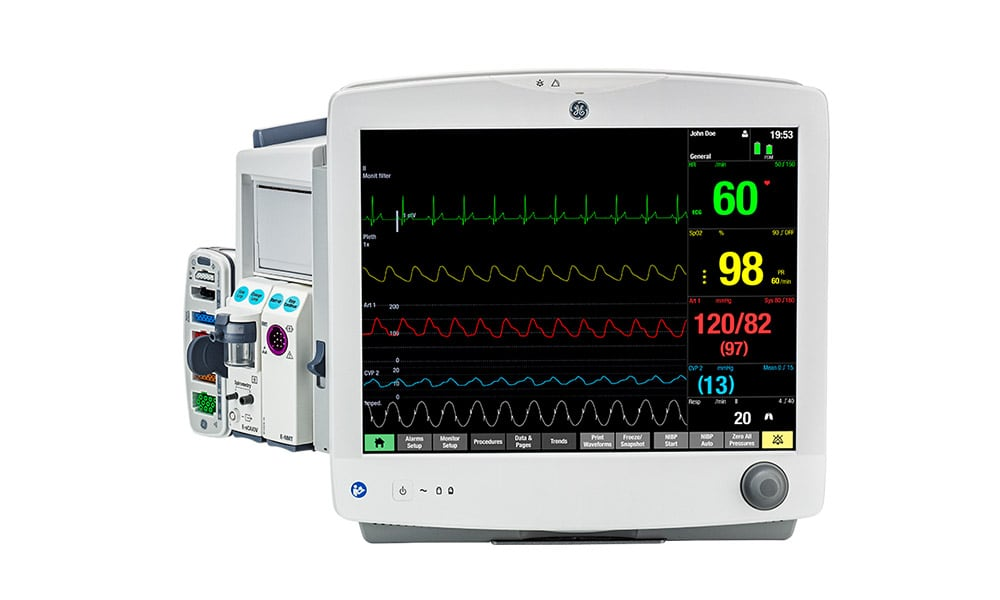
\includegraphics[width=7cm]{pulse_preprocess/monitor1}
    }
    \quad
    \subfigure[B650监护界面]{
    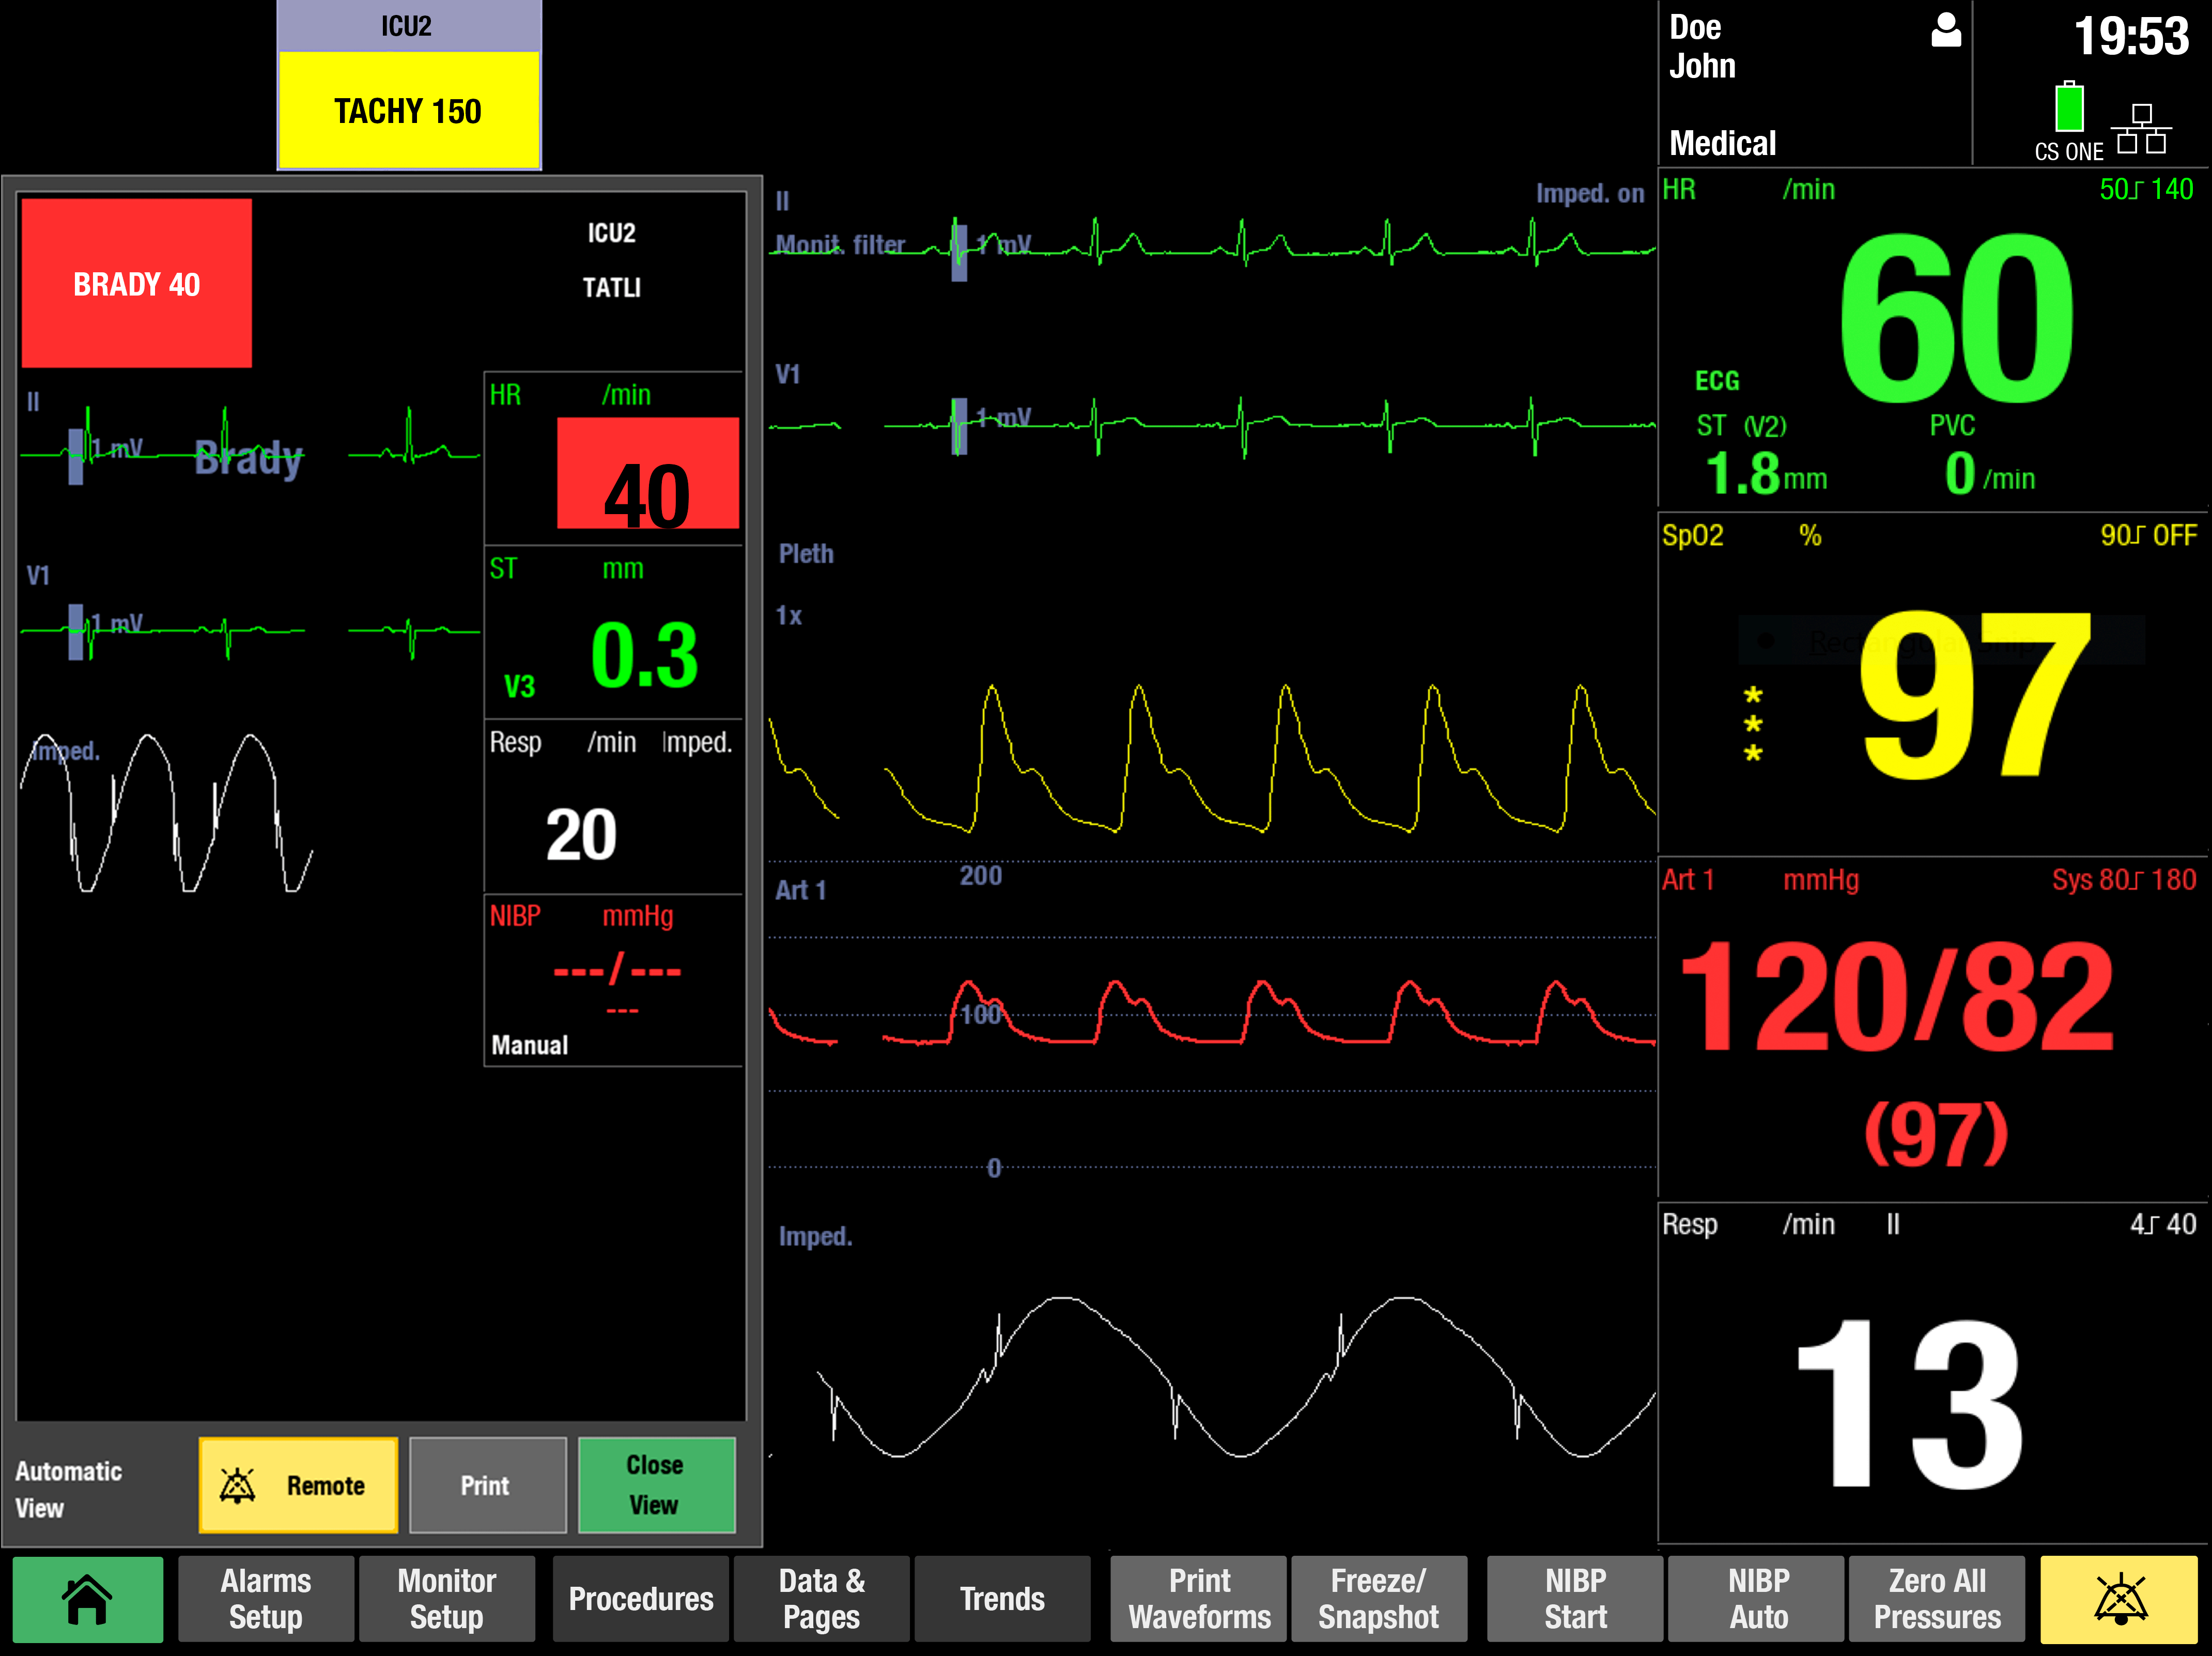
\includegraphics[width=5.5cm]{pulse_preprocess/monitor2}
    }
    \caption{\label{fig:monitor}美国GE公司的Healthcare CARESCAPE B650监护仪示意图}
\end{figure}

此外,本研究选择了美国Tyco公司的Nellcor DS-100A型透射式血氧传感器作为B650型的配套组件,如\autoref{fig:ds100a}所示。
该传感器一般佩戴在被试左手食指上,若被试的左手食指有损伤,则将测量部位替换为左手中指。
在测量时,手指需放入传感器指套内部,使指甲与传感器表面有指甲标记的部位正对,指尖触及但不超出指套顶端,以确保发光管发出的所有光线全部通过被试的组织。

\begin{figure}[htbp]
    \centering
    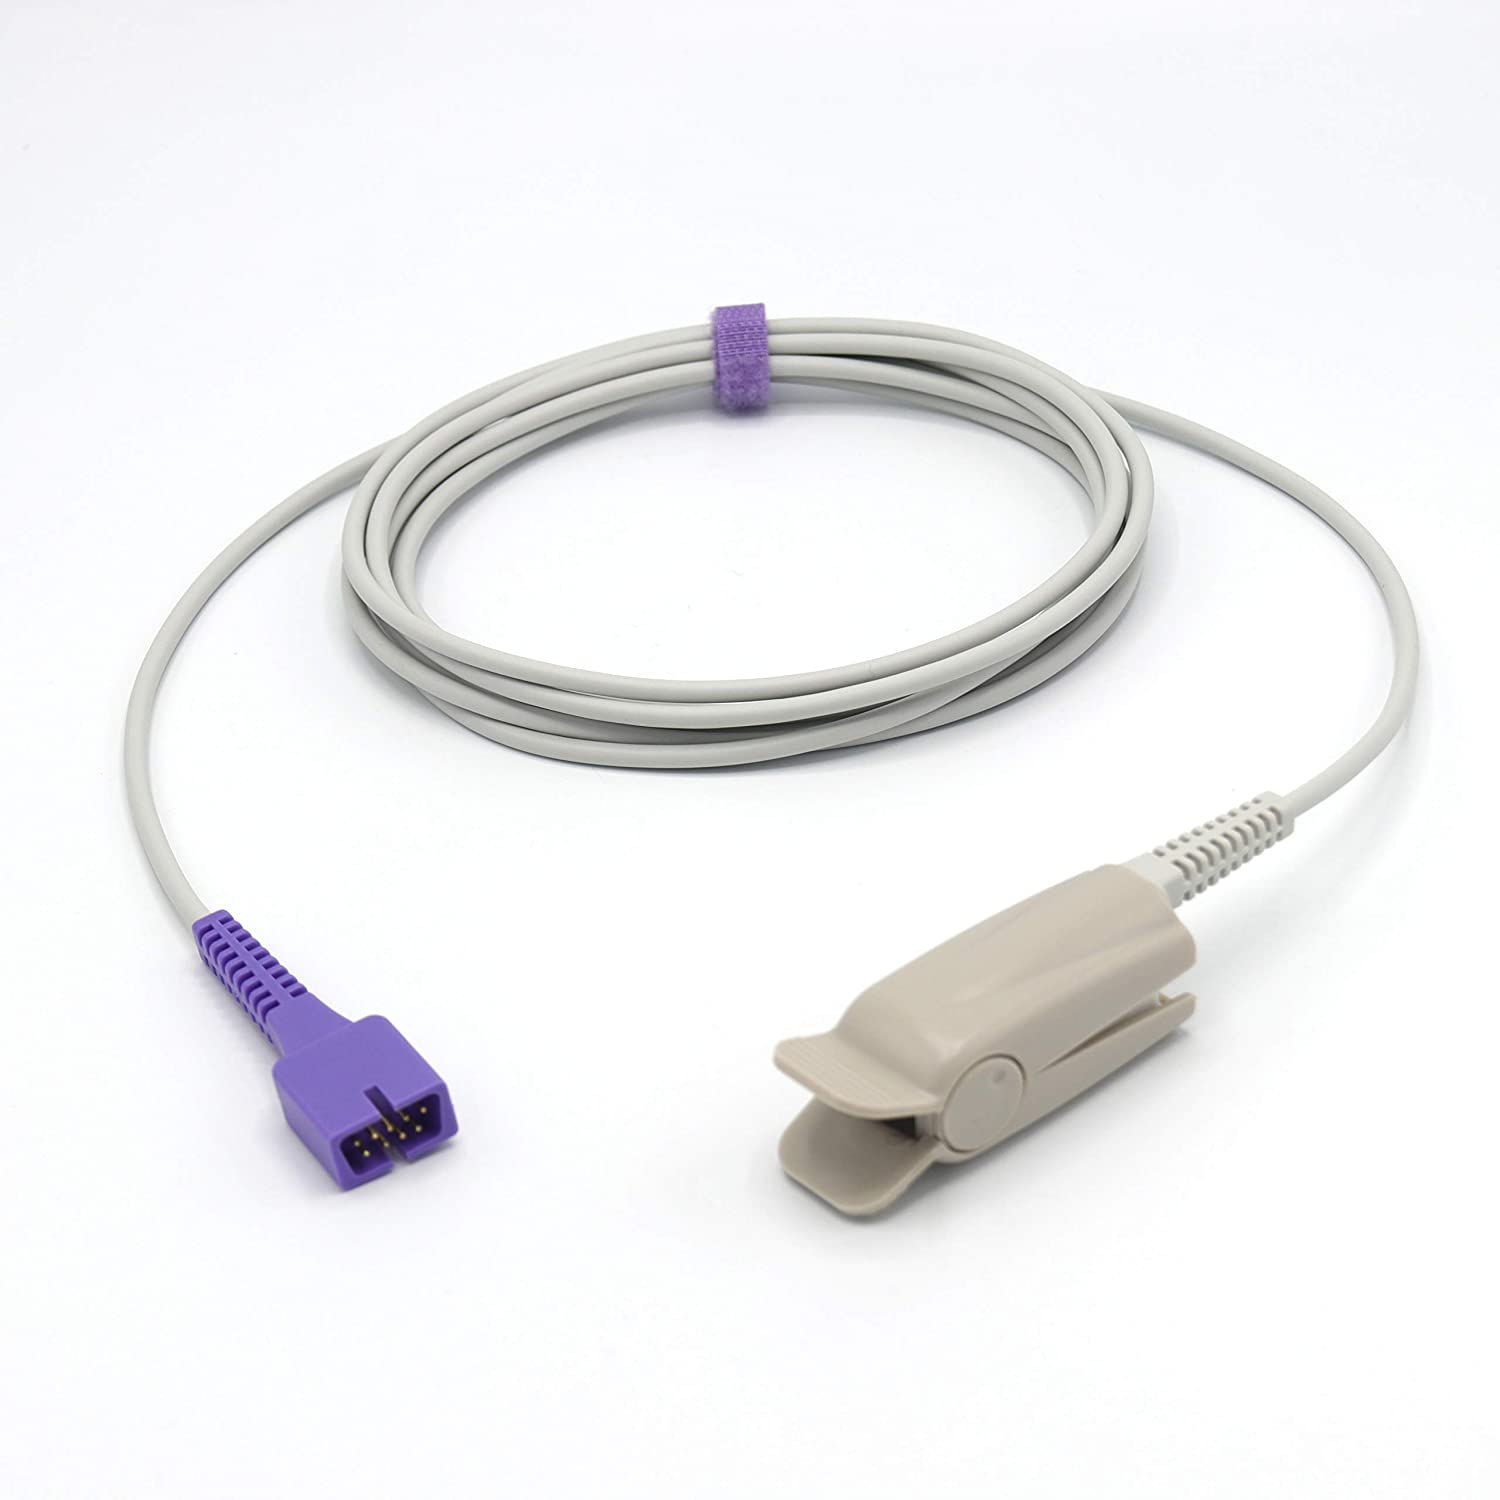
\includegraphics[width=0.4\linewidth]{pulse_preprocess/ds100a}
    \caption{\label{fig:ds100a}美国Tyco公司的Nellcor DS-100A型血氧传感器示意图}
\end{figure}

\subsection{实验流程}
被试到达实验场地后,由实验人员登记其PE风险因子信息,包括姓名、年龄、孕产史等。接着实验人员会告知被试本实验的研究目的与具体实验流程。
在征得被试同意后,实验人员按操作规范为被试佩戴血氧采集探头\cite{Chen2021}。
在被试休息至少5min后,开始进行PPG数据采集,单次采集时长不少于1min。被试需在实验全程中保持坐姿,禁止说话发声或产生较大的肢体动作。

\subsection{数据导出及复核}
由于美国GE公司未公开B650型监护仪的数据通讯协议,本研究无法直接获取该设备全部生理参数的原始数据。最后通过技术产商提供的第三方软件,将PPG原始数据以
(时间,相对幅值)的键值对的形式以逗号分隔值(comma-separated values,CSV)文件格式导出,导出的PPG信号采样率为100Hz。

本研究共采集得到了80例被试的PPG原始数据。经复核校验,1例正常妊娠的被试数据因采集时间过短、信号质量过低被剔除,
剩余79例为有效数据,包括44例实验组数据和35例对照组数据。

\section{被试孕妇人口统计学特征分析}
本节使用统计分析方法对上述实验中被试的年龄、孕周、身高、体重、BMI指数、血压及心率等人口统计学特征进行了相关性分析。

\subsection{变量分析方法}
相关性分析和参数检验与非参数检验是统计分析学科中最常用的工具,本小节对相关性分析方法的原理进行介绍,同时着重介绍了非参数检验的原理及方法。

一、相关性分析

相关性分析(correlation analysis,CA)是对两个具备相关性的变量元素进行分析,衡量这两个变量因素的相关密切程度\cite{Zhang2019}。这两个变量元素之间需要存在一定的联系才可以进行相关性分析。

\begin{figure}[htbp]
    \centering
    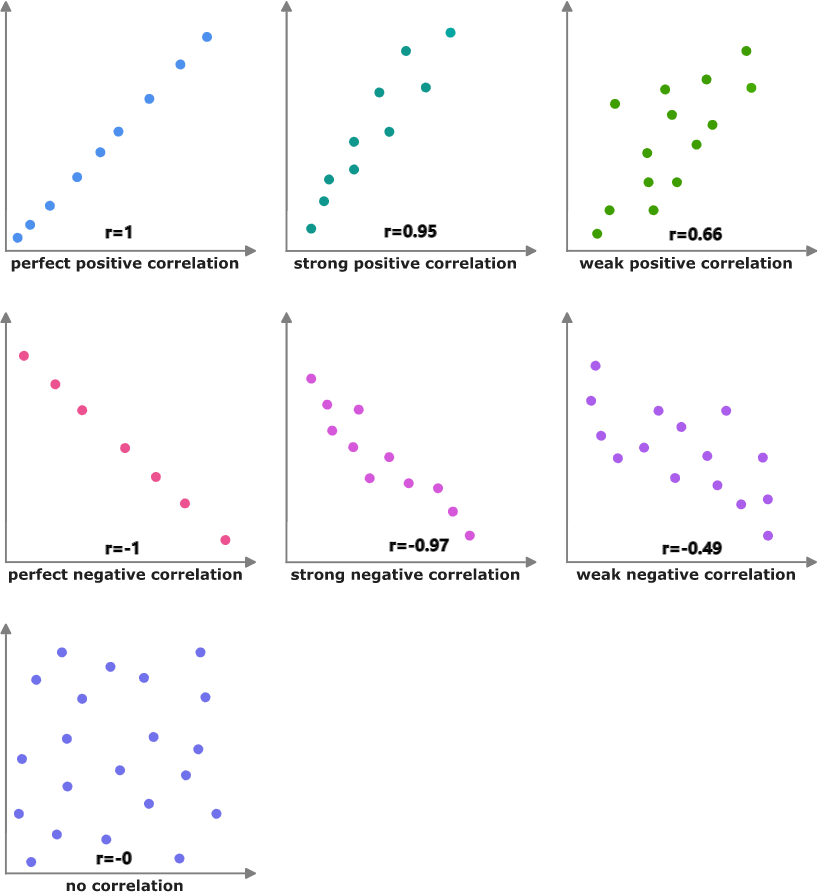
\includegraphics[width=.6\linewidth]{pulse_preprocess/relation}
    \caption[二元变量相关关系示意图]{\label{fig:relation}二元变量相关关系示意图\cite{IXL2022}}
\end{figure}

统计学上引入了相关系数$r$以量化表征变量之间的密切程度。$r$的取值范围为[-1,1],其绝对值大小反映了两变量之间相关性的强弱:当$r$>0时,表明两个变量正相关;反之,则两个变量变化趋势相反,呈负相关。
可以通过散点图直接观察两个变量之间的联系,如\autoref{fig:relation}所示,两个变量的$r$值也在每副子图中进行了标注。

常用的相关性分析方法有皮尔逊(Pearson)相关性分析法与斯皮尔曼(Spearman)相关性分析法,利用这两种方法可分别得到皮尔逊相关系数$r_p$与斯皮尔曼相关系数$r_s$
\begin{equation}
    \label{equ:spearman}
    r_s=1-\frac{6\sum_{i=1}^{n}(x_{i}-y_{i})^2}{n(n^2-1)}
\end{equation}
\begin{equation}
    \label{equ:pearson}
    r_p=\frac{\sum_{i=1}^n{(x_i- \mathop{x} \limits^-)(y_i- \mathop{y} \limits^-)}}{\sqrt{{\sum_{i=1}^n}{{(x_i- \mathop{x} \limits^-)^2\sum_{i=1}^n}{(y_i- \mathop{y} \limits^-)^2}}}}
\end{equation}

一般认为,斯皮尔曼相关性分析适用于对存在单调性关系的变量进行检测,而皮尔逊相关性分析适用于对满足正态分布的变量进行检测。
相较而言,斯皮尔曼相关系数对变量的分布特性要求并不严格,应用得也更为广泛。

为计算斯皮尔曼相关系数,需要对长度为$n$的待检二元变量$X$与$Y$按升序排列,得到原始数据在排序后的序次$x$、$y$,通过序次$x$、$y$完成计算。
若出现多个数据排序相同,则用这些数据的平均序次统一表征后再进行计算,如\autoref{equ:spearman}所示。

二、参数检验与非参数检验

数据的集中趋势、离散程度与分布形态是对描述一组数据时最常用的三个统计指标。参数检验(parametric test,PT)通常是在假设数据总体服从正态分布、
样本统计量服从T分布的前提下,对总体分布中的未知的总体均值、方差及样本差等参数做出统计推断。
而面对总体分布类型未知或分布类型已知,但不对称或变量无法精准测量的数据,或样本容量小、无法运用中心极限定理,
参数检验方法均无法处理。因此,
另一类不以特定的总体分布为前提、不针对总体分布参数做任何推断的分析方法也发展起来,此类分析方法被统一称为非参数检验(non-parametric test,NPT)\cite{Guo2017,Zhang2019}。

一般而言,参数检验的精确度高于非参数检验,因此在条件允许的情况下,应优先采用参数检验。若由于各种原因导致参数检验的条件不满足,可以应用非参数检验方法对数据进行分析。
常见的非参数检验方法及其适用情形如\autoref{tab:nonparametric-test}所示。
\begin{longtblr}
    [
        theme          = {zju},
        caption        = {常见的非参数检验方法},
        label          = {tab:nonparametric-test},
    ]
    {
        colspec        = {X[1,c,m]X[1.8,c,m]X[2,c,m]X[4.5,c,m]X[4.5,c,m]},
        hline{1,Z}     = {\thickline},
        hline{2}       = {\thinline},
        rowhead        = 1,
        row{1}         = {font=\headfont},
        row{2-Z}       = {font=\nonheadfont},
    }
    序号 & 样本数目 & 样本相关性 & 检验方法 & 检验方法英文名 \\
    1  & 单样本   & /     & 卡方检验  & Chi-Squared Test \\
    2  & 单样本   & /     & 二项分布检验 & Binomial Test \\
    3  & 单样本   & /     & K-S检验 & Kolmogorov–Smirnov Test \\
    4  & 单样本   & /     & 符号秩检验 & Wilcoxon Signed-Rank Test \\
    5  & 单样本   & /     & 游程检验  & Wald–Wolfowitz runs Test \\
    6  & 两样本   & 独立    & Wilcxon W等级和检验 & Mann-Whitney U Test \\
    7  & 两样本   & 独立    & 摩西极端反映差异检验 & Moses Extreme Reaction Test \\
    8  & 两样本   & 独立    & K-S检验 & Kolmogorov–Smirnov Test \\
    9  & 两样本   & 独立    & 游程检验  & Wald–Wolfowitz runs Test \\
    10  & 两样本   & 相关    & 符号检验  & Sign Test \\
    11  & 两样本   & 相关    & 符号秩检验 & Wilcoxon Signed-Rank Test \\
    12  & 两样本   & 相关    & 变化显著性检验 & McNemar's Test \\
    13  & 两样本   & 相关    & 边缘一致性检验 & Marginal Homogeneity Test \\
    14  & 多样本   & 独立    & K-W平均秩检验 & Kruskal-Wallis H Test \\
    15  & 多样本   & 独立    & 中位数检验 & Median Test \\
    16  & 多样本   & 独立    & 分组分布检验 & Jonckheere-Terpstra Test \\
    17  & 多样本   & 相关    & 双向等级方差分析 & Friedman Test \\
    18  & 多样本   & 相关    & 肯德尔和谐系数检验 & Kendall's W Test \\
    19  & 多样本   & 相关    & 二分变量检验 & Cochran's Q Test \\
\end{longtblr}

\subsection{分析结果}
由于通过临床数据实验得到的被试人口统计学特征、PE风险因子等待检参数存在样本量较小、具体分布未知等客观限制因素,不满足参数检验的条件。
本研究最终从\autoref{tab:nonparametric-test}中选取了Wilcxon W等级和检验方法,亦即Mann-Whitney U检验对被试的人口统计学特征、PE风险因子在实验室与对照组上
是否存在分布差异进行了相关性分析。

U检验的基本思想是将全部样本混合后一起求秩,然后根据两组样本的秩分情况判断是否存在差异。
上述待检变量经U检验后的结果如\autoref{tab:factors_res}所示。其中,所有待检变量均以(平均值±标准差)的形式表征,组别之间存在分布差异的变量
进行了特殊标注。

\begin{longtblr}
    [
        theme          = {zju},
        caption        = {被试孕妇风险因子统计结果},
        label          = {tab:factors_res},
        note{*}        = {有统计意义上的显著性区别。},
    ]
    {
        colspec        = {X[1,c,m]X[3.5,c,m]X[3.5,c,m]X[3.5,c,m]X[2,c,m]},
        hline{1,Z}     = {\thickline},
        hline{2}       = {\thinline},
        rowhead        = 1,
        row{1}         = {font=\headfont},
        row{2-Z}       = {font=\nonheadfont},
    }
    序号 & 检验变量(单位) & 实验组(n=44) & 对照组(n=35) & $p$值 \\
    1 & 年龄(years) & 32.3±3.6 & 33.8±4.6 & 0.108 \\
    2 & 孕周(weeks) & 32.7±3.8 & 34.3±4.3 & 0.053 \\
    3 & 身高(cm) & 158.1±5.0 & 160.0±3.3 & 0.089 \\
    4 & 体重(kg) &  75.7±12.9 &  67.1±8.2 & 0.002\TblrNote{*} \\
    5 & BMI(kg/cm) &  30.2±4.5 &  26.2±3.3 & <0.001\TblrNote{*}\\
    6 & 收缩压(mmhg) &  160.1±19.5 &  111.2±9.8 & <0.001\TblrNote{*} \\
    7 & 舒张压(mmhg) &  96.1±14.5 &  66.8±10.4 & <0.001\TblrNote{*} \\
    8 & 心率(bpm) & 87.0±11.9 & 87.5±13.1 & 0.656 \\
\end{longtblr}

从\autoref{tab:factors_res}可以发现,实验组与对照组的被试孕妇在年龄、孕周、身高、心率等风险因子
上均无明显统计意义上的差别($p$>0.05),但在收缩压与舒张压的数值上有显著差异($p$<0.001),这也与被试孕妇的PE病发状态一致,符合预期。

\section{脉搏波的预处理}
不同硬件设备采集的PPG数据在采样率、采样精度及导出的数据格式等方面存在着一定的差异,同时这些设备对数据采集过程中出现的人体肌电、呼吸与体动以及环境工频等噪声干扰的软硬件滤波处理能力也不尽相同。
因此,在对PPG进行分析前,通常需要进行一定的数据预处理。

\begin{figure}[htbp]
    \centering
    \includegraphics[width=0.8\linewidth]{pulse_preprocess/samplesignal}
    \caption{\label{fig:samplesignal}临床数据实验采集得到的PPG信号示意图}
\end{figure}

\autoref{fig:samplesignal}展示了本研究临床数据实验采集得到的一段有代表性的PPG数据波形。
从\autoref{fig:samplesignal}中可以看到,本次临床数据实验经由GE B650型监护仪采集得到的PPG信号质量较高,但仍然存在着基线偏移、PPG信号重搏波特征不明显等问题。这些问题可能与实验使用的传感器种类、监护仪硬件检测电路及监护仪软件处理算法等因素有关。
另一方面,如\autoref{fig:samplesignal}框选部分所示,40s至55s内存在着一段无效干扰数据,在进行分析前必须设法对其进行剔除。

本节将具体介绍对PPG信号的分析预处理过程,同时说明预处理各过程中使用的具体算法。PPG预处理过程包括滤波处理、波形检测、去除基线漂移、信号重采样与数据标准化等,如\autoref{fig:process}所示。
其中,着重介绍了本研究提出的一种可在多平台、多研究背景下应用的新型PPG波形检测算法。
\begin{figure}[htbp]
    \centering
    
\includegraphics[width=0.5\linewidth]{pulse_preprocess/process}
    \caption{\label{fig:process}PPG预处理流程示意图}
\end{figure}

\subsection{信号滤波}
数字滤波可从原始信号获取特定频段的成分,是信号处理的常见的处理方法。而在人体电生理信号分析领域,数字滤波更是必不可少的处理步骤。针对人体各电生理信号,此前的诸多学者们提出了多种不同的滤波算法。
由于如\autoref{fig:samplesignal}所示的原始PPG信号质量高、干扰噪声较少,本研究仅使用较为简单的平均滑动滤波器对其进行了处理。

平滑滤波器本质上是一个低通滤波器,若以$X$表示原始信号,$Y$表示滤波后信号,$N$表示其滤波阶数,则平滑滤波过程可表示为
\begin{equation}
    \label{equ:filter}
    Y(k)=\frac{1}{N}\sum_{i=0}^{N-1}X(k+i)
\end{equation}
而该滤波器的截止频率(cutoff frequency,CF)与滤波阶数$N$存在以下关系\cite{malp2011}
\begin{equation}
    \label{equ:malpf}
    f_{c} \approx 0.443 \cdot \frac{f_s}{N}    
\end{equation}
其中,$f_s$为原始信号采样率。由\autoref{equ:malpf}可知,滤波器的阶数越高,其CF越低,滤波后信号越均匀平滑,滤波效果越好。

另一方面,信噪比(signal-noise rate,SNR)与均方误差(root mean square error,RMSE)是最常用的评估滤波效果优劣的两个指标,其定义分别为
\begin{equation}
    \label{equ:snr}
    \text{SNR}=10 \cdot \log_{10}\frac{\sum_{i=1}^{n}{(X_i-\mathop{X} \limits^-})^2}{\sum_{i=1}^{n}{(X_i-Y_i})^2}
\end{equation}
\begin{equation}
    \label{equ:rmse}
    \text{RMSE}=\sqrt{\frac{\sum_{i=1}^{n}{(X_i-Y_i})^2}{n}}
\end{equation}

\begin{figure}[htbp]
    \centering
    \subfigure[原始PPG信号示意图]{
    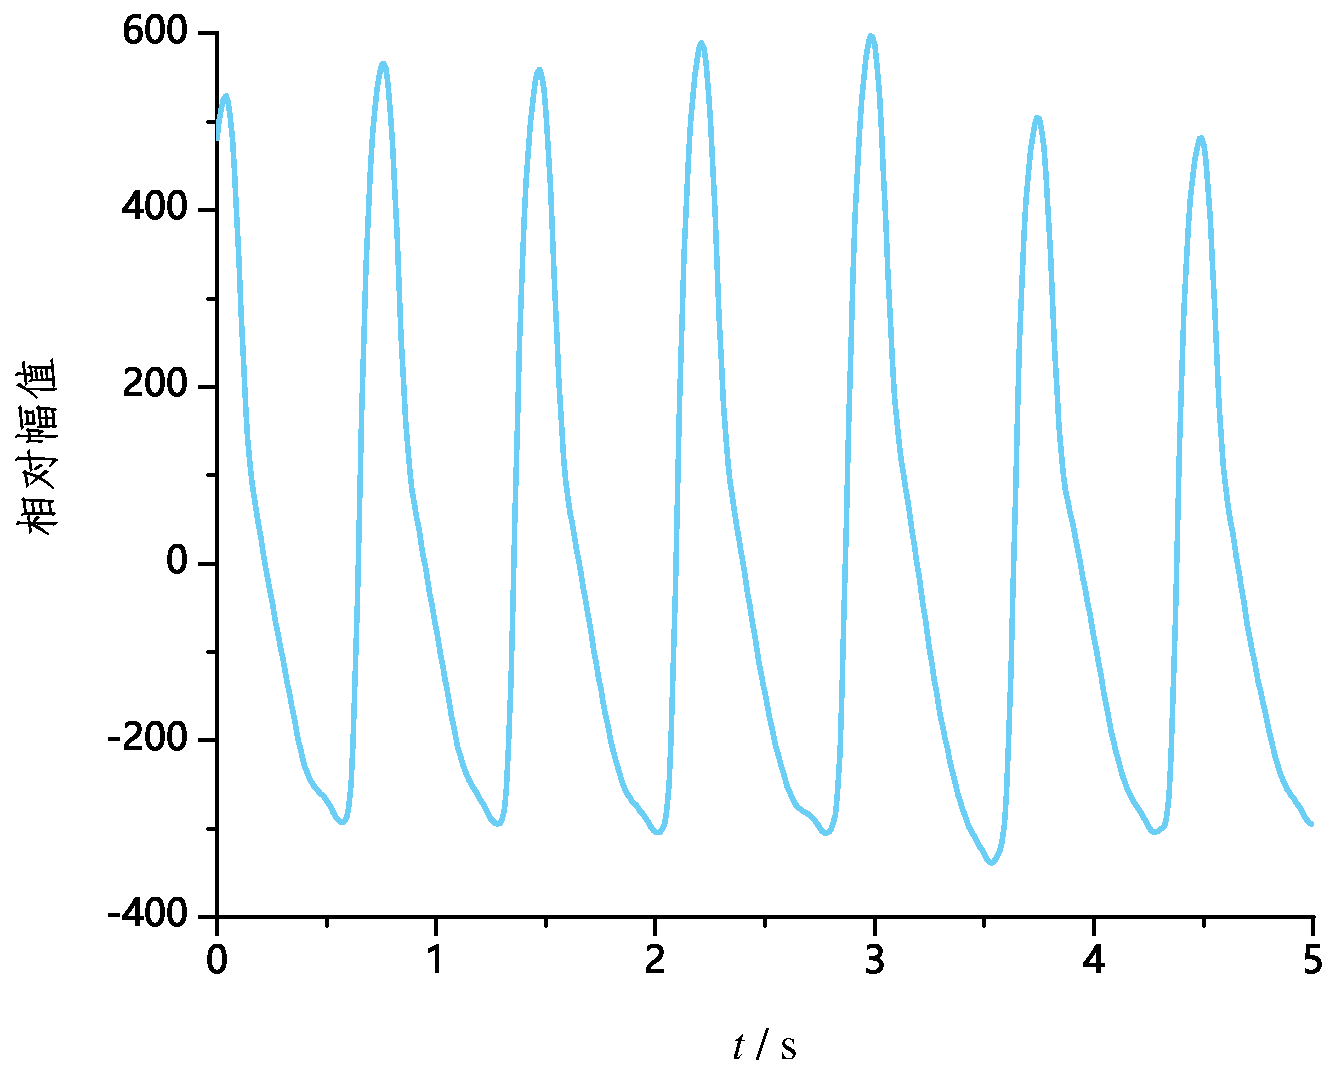
\includegraphics[width=6.5cm]{pulse_preprocess/before_filter}
    }
    \quad
    \subfigure[平滑滤波后PPG信号示意图]{
    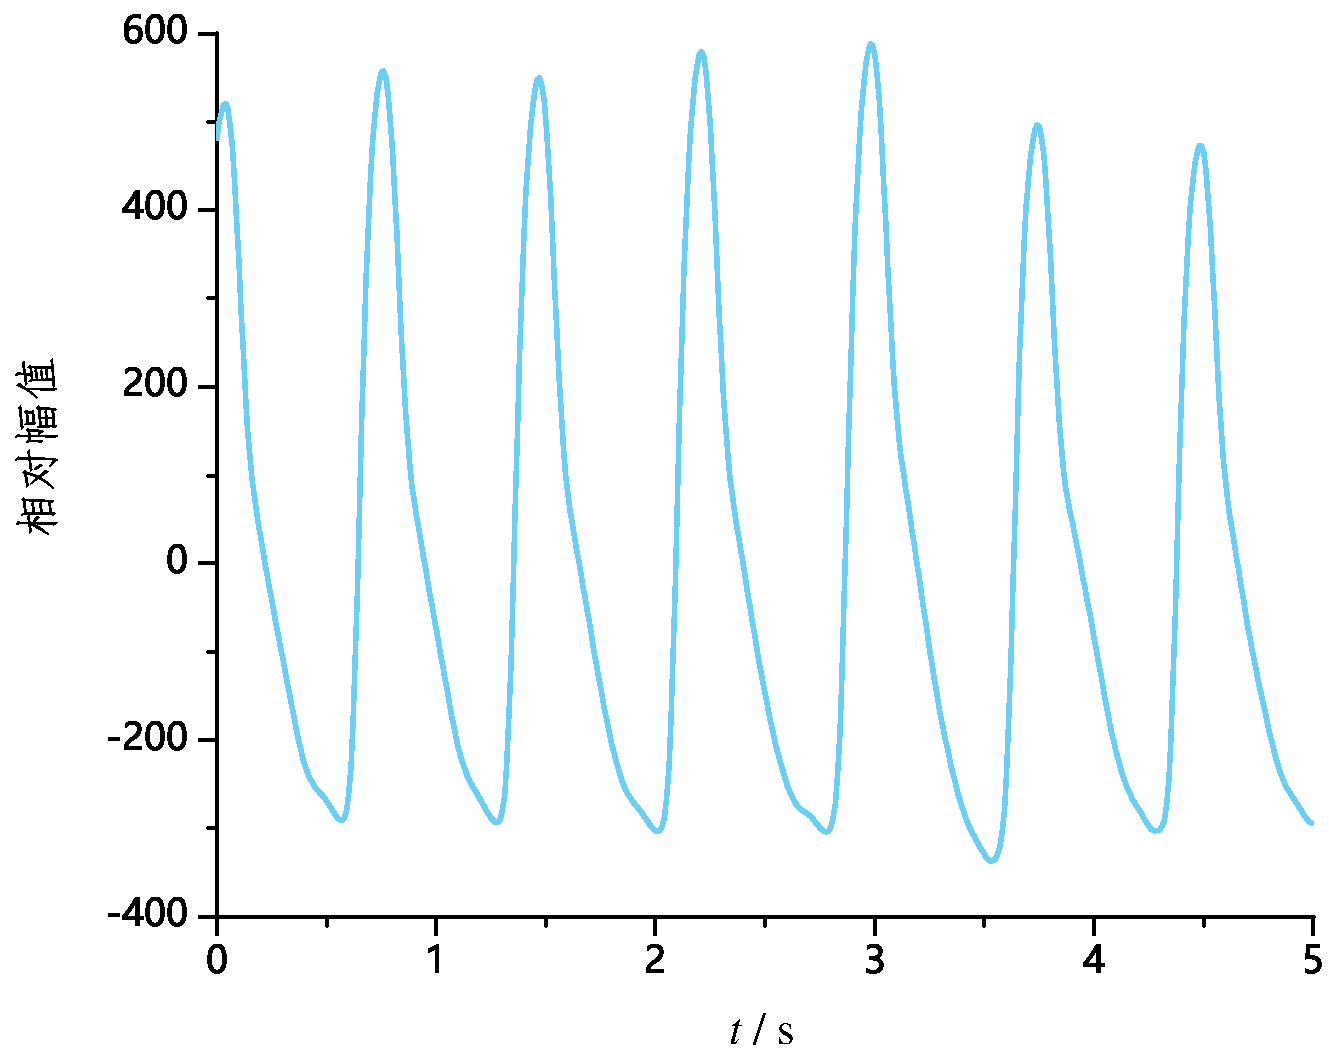
\includegraphics[width=6.5cm]{pulse_preprocess/after_filter}
    }
    \caption{\label{fig:filter}平滑滤波前后PPG信号对比图}
\end{figure}

本论文使用了$N$=5的平滑滤波器对原始PPG信号进行处理,滤波前后对比如\autoref{fig:filter}所示。
由\autoref{equ:malpf}可知,此时滤波器对应的的截止频率约为8.9Hz。
通过SNR与RMSE评估\autoref{fig:filter}中的效果,可得$\text{SNR}$=33.19,$\text{RMSE}$=6.27。
这说明PPG信号波形特征已比较清晰,因此,滤波阶数$N$为5的平滑滤波器可满足后续分析需求。

\subsection{波形检测}
准确地检测PPG波形是分析研究的前提。多数PPG波形检测算法一般会一次性完成PPG波形的分析与检测,而对检测结果的校验需全部由人工完成\cite{Zhang2010,Chen2021,Allen2007,Feng2018,FengJiang2018}。
在处理受到干扰或存在畸变的PPG数据时,此类算法的检测性能通常也会下降。
为改进这些问题,在借鉴计算机科学领域的策略与机制分离思想的基础上\cite{Levin1975},本研究对PPG波形的检测过程进行了模式设计,
提出一种基于初筛—复核—决策(screening-checking-deciding,SCD)的新型算法,其处理流程如\autoref{fig:detect}所示。

\begin{figure}[htbp]
    \centering
    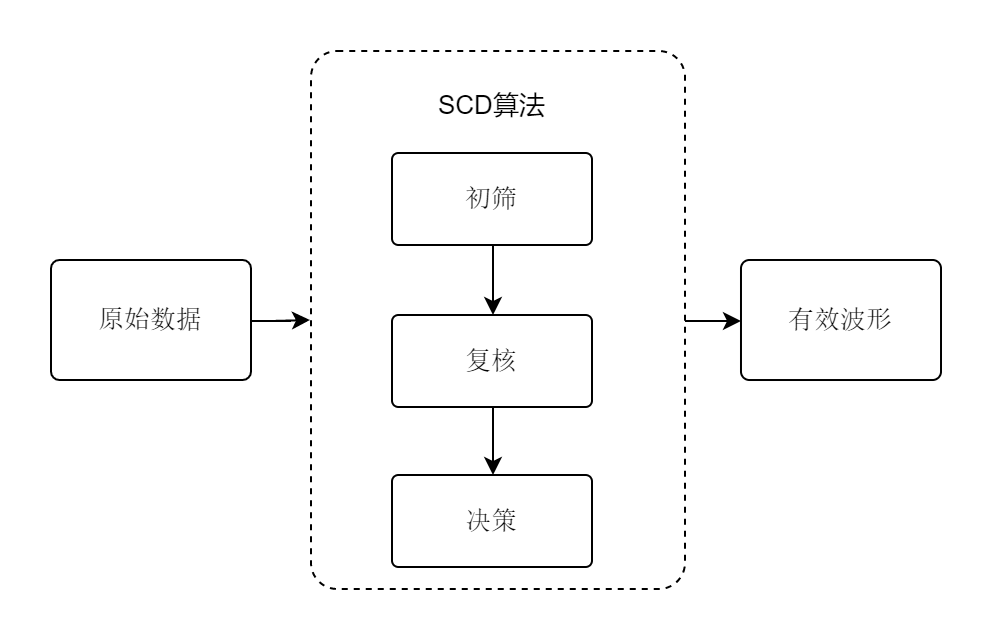
\includegraphics[width=0.65\linewidth]{pulse_preprocess/scd}
    \caption{\label{fig:detect}SCD算法检测流程示意图}
\end{figure}

机制与策略分离是计算机系统领域的一项重要设计原则,被广泛应用于一系列资源分配问题(如CPU调度、内存分配、服务质量)以及软件抽象的设计等问题中\cite{Levin1975}。
这里的机制可以理解成决定如何做(how),而策略则决定具体做什么(what)。
SCD算法以“宽进严出”为原则,通过初筛、复核及决策等机制检测有效PPG波形。
其中,初筛阶段可初步确定PPG波形;复核阶段利用多种形态学特征,将初筛结果定性描述为有效波形或异常干扰;决策阶段则是按照一定的策略从上述定性描述中最终确定有效波形。
SCD算法对各机制下使用的具体策略不做过多限制,支持直接更改初筛算法,增删复核标准,切换决策策略等设置。
这保证了SCD算法的适用性与调整的灵活性,使高效准确地检测受到干扰或存在畸变的PPG数据成为可能。
以下是对SCD算法的详细介绍。

一、超参数

SCD算法可以视为一个广义上的监督学习模型的训练与应用过程\cite{Zhou2016}。其中,多种形态学特征的复核结果对应着模型的输入数据,决策阶段使用的策略对应着模型的训练算法,
确定有效波形的决策过程则对应着模型在新数据集上的应用过程。而初筛、复核与决策阶段涉及的多项具体数值可以视为该模型的超参数。

对一个监督学习来说,其模型超参数的训练依赖于训练集数据,并需要观察模型对测试集中数据标签的预测结果进行反馈调整\cite{Zhou2016}。
而在SCD算法的超参数调参过程中,本研究基于自主实验的部分数据确定了训练集,得到了这些超参数的具体数值(参见3.2小节)。
特别地,对SCD算法的校验还需要结合波形的具体形态,尤其是畸变波形的形态。这是由于畸变波形的正确识别与否直接影响了SCD算法的整体识别准确率。

二、初筛

波峰与波谷是脉搏波的最基本特征点,也是检测波形其他特征点的基础。在初筛阶段,SCD算法通过搜索窗定位PPG的波峰与波谷,再从原始数据中确定波形。

1、波峰定位

波峰是特定PPG波形内的最大值,在其左邻域内PPG幅值单调递增,右邻域内PPG幅值单调递减,则显然波峰必然是原始数据中的局部极大值。

本研究使用的波峰的定位步骤如下:

1)计算并遍历原始信号的一阶导数$x^{'}$,若出现$x_i^{'}\ge 0$且$x_{i+1}^{'}\le 0$,则说明出现了极大值。

2)定义一长一短的两个搜索窗,分别以当前数据点为窗中心,向前后双向检测并返回窗内最大值的位置。

3)若两个搜索窗的返回结果一致,则说明返回值就是一个波峰点。为防止同一波峰被多次检测,只有与上一成功检测的波峰位置点不同返回值才会被加入波峰缓存数组$Peaks$中。

在实际检测时,常会出现一阶导数在某邻域内多次出现过零点,导致多个局部极大值连续出现。为避免连续调用搜索窗、提高算法效率,本研究针对性进行了以下剪枝优化设计:

1)采用中心对称搜索窗

窗口进行最大值搜索时是以当前搜索位置中心对称前后双向搜索,当第一个过零点出现时,这一邻域内的所有极值点均已被检索过,得到的局部最值已经是该邻域内最大值。

2)合理设置搜索窗时长

结合正常波形的形态特点,本研究将搜索窗时长分别设置为0.1s与0.3s。前者可以直接剔除掉时间跨度过小的局部极值,后者是基于此前PPG波峰与其重搏峰时间间隔的经验值,可以保证重搏峰点不会被误检为整个波形的波峰。

3)搜索窗步进值策略调整

若长窗在当前位置$C$以中心沿时间轴延伸方向找到了局部极大值的坐标$L$后,下一次的搜索窗位置可直接从该$L$处开始。当搜索完成后,若短窗返回结果$S=L$,则返回值必然是检测得到的波峰位置$P$,下次搜索可直接从波峰后开始;若$S\ne L$,
此时从$C$至$L$再进行搜索已经不可能再更新$L$坐标。而由于长窗搜索必然包含短窗,故下次搜索也可以同样调整检索位置从$L$处开始。

2、波谷定位

在波峰的位置确定之后,波谷的定位相对简单,一种可行的处理思路是将两个连续波峰之间的最小值定义为PPG波形的波谷。但该思路已同时默认波形之间有连续性,即任意两个波形之间不存在其他干扰段,
且所有的波峰均已被正确无误地检测出来。因此,这种思路无法对复杂信号进行有效处理。

本研究改进了上述思路,对波谷的定位按照先寻找定位再二次确认的方法进行。除满足最小值的条件下,波谷需要进一步满足其出现位置必须在这两个波峰之间的后半段。
此步得到的PPG波谷位置也被保存至缓存数组$Troughs$中,这一过程如\autoref{alg:troughs_detect}所示。
\begin{breakablealgorithm}
    \caption{PPG波形波谷定位检测}
    \label{alg:troughs_detect}
    \begin{algorithmic}[1] %每行显示行号
        \Require 待检原始数据数组$Points$,原始数据的一阶差分数组$D$,波峰数组$Peaks$
        \Ensure 正常形态下记录脉搏波波谷位置的数组
        \Function {DetectTroughs}{$Points, D, Peaks$}
            \State 初始化$Troughs$
            \For{$i\gets 0,Peaks.length()-1$}
                \State $leastX \gets (Peaks[i].x + Peaks[i+1].x )/2$
                    \For{$j \gets Peaks[i+1].x)-1, leastX$}
                        \If {$D[j-1]<0 \And D[j]\le 0$}
                            \State $lastT \gets Points[j]$
                            \State \textbf{break}
                        \EndIf
                    \EndFor
                \State $Troughs \gets lastT$
            \EndFor
            \State \Return{$Troughs$}
        \EndFunction
    \end{algorithmic}
\end{breakablealgorithm}

3、完整波形确认

此前两步已经分别得到了原始信号中所有波峰与波谷点,此时仅需按照(波谷,波峰,下一波谷)的规则组合成完整波形即可。
但对某些异常信号,\autoref{alg:troughs_detect}无法有效检出在两波峰的波谷。
因此,有必要组合后的波形再次进行检查校对。

参考以往研究对PPG波形对经验统计,本研究以一定的PPG波形的时间规则完成校对,以确保有效波形的必定在这些时间规则规定的间期内。
这些时间规则包括,波形起点与波形终点间期需要$P_{S2E}$需要大于0.4s,波形峰值点与波形终点间期$P_{P2E}$需要大于0.3s。

4、其他特征点定位

初筛阶段不做除波峰波谷外的其他特征点检测。其他特征点的定位依赖于波形的正确检测,这些检测被推迟到SCD算法检测完成后才进行。

三、复核

由于PPG是一种平稳随机信号,短时间内采样得到的数据波形理应具有较高的相似度\cite{Qiu2012}。
而有效PPG波形与干扰、畸变信号在形态特征、统计特征上往往存在着一定差异,存在通过软件算法进行智能识别区分的理论可行性。
因此,SCD算法设计了PPG波形的多种形态学特征,并以这些特征为标准对初筛结果进行复核。

1、功率

功率标准描述了PPG波形的能量均值,也即波形内所有采样点的幅值平方的均值
\begin{equation}
    \label{equ:ppgp}
    P=\frac{\sum_{i=0}^{n-1}{x_i}^2}{n}
\end{equation}

其中,$P$为当前PPG波形功率值,$n$为该波形的采样点数,$x_i$为该波形每个采样点的采样幅值。

2、标准差

标准差标准描述了PPG波形中交流成分的平均幅值,是对上述功率标准的补充
\begin{equation}
    \label{equ:ppgstd}
    S=\sqrt{\frac{\sum_{i=0}^{n-1}{(x_i-\mathop{x} \limits^-})^2}{n}}
\end{equation}

其中,$S$为当前PPG波形功率值,$n$为该波形的采样点数,$x_i$为该波形每个采样点的幅值, $\mathop{x} \limits^-$为该波形内所有采样点的幅值均值。

3、波峰相对位置 

由于血管回流作用,PPG波形的下降支会较上升支持续时间更长,波峰必然出现在PPG波形的前半段。而波峰在PPG波形的相对位置可表示为
\begin{equation}
    \label{equ:rpeak}
    R = \frac{n}{n_p}
\end{equation}

其中,$R$为当前PPG波形的波峰相对位置,$n$为该波形的采样点数,$n_p$为该波形波峰所对应的采样点下标值。

4、基线漂移程度 

基线漂移程度衡量了PPG波形起点与终点幅值差异,可量化PPG波形受到干扰的程度,可用下列公式衡量
\begin{equation}
    \label{equ:b1}
    B_1 = |x_s-x_e|
\end{equation}
\begin{equation}
    \label{equ:b2}
    B_2 = \frac{|x_s-x_e|}{|x_p-x_l|}
\end{equation}
\begin{equation}
    \label{equ:b3}
    B_3 = \frac{x_p-x_s}{x_p-x_e}
\end{equation}

其中,$B_1$是对当前PPG波形的基线漂移程度绝对数值衡量,$B_2$与$B_3$是对当前PPG波形的基线漂移两种相对数值衡量。而$x_p$、$x_s$与$x_e$分别为PPG的波峰、起点与终点处幅值,
$x_l$为$x_s$与$x_e$中数值较小者。

5、其他标准

由于不同人群、不同采集设备、不同采集环境下采集得到的PPG信号可能形态上千差万别,与之对应的干扰信号也往往不尽相同。上述标准仍有不足以甄别区分有效信号与无效干扰的可能。
故SCD算法允许根据实际分析需要,自习定义新的复核标准或只使用以上部分复核标准。

另外,与PPG波形相关的时间标准也多次在SCD算法中得到应用。
在初筛时,搜索窗的窗长已经限定了重搏波峰与主波峰间期$T_{P2R}$需要大于0.3s;
完整波形在进行确认时也限定了波形周期$T_{S2E}$需要大于0.4s、下降支时长$P_{P2E}$需要大于0.3s。
若参照心率定义,将每分钟内有效脉搏波的数量规定为脉率(pulse rate,PR),原则上SCD算法可对$PR \le$150的PPG数据进行波形检测。

6、有效波形判断

复核阶段进行有效波形判断时,使用的是上述PPG的形态学特征基于数值比较的逻辑值,而非其具体数值。
这是由于PPG波形个体差异性较为明显;同时,在上述特征上,同一个体的有效PPG波形与干扰、畸变信号也存在着较为显著的数值差异。
使用具体特征标准进行复核的步骤如下:

1)计算当前个体的所有PPG波形对应的特征值。

2)将步骤1中所有数值排序后,选取部分数值计算均值。

3)依次将所有特征值与该均值进行比较,若特征值在均值的一定区间内,对应的波形才会被判断为有效波形(输出0);否则会被判为异常干扰(输出1)。

复核阶段的超参数数值如\autoref{tab:checkingp}所示。

\begin{longtblr}
    [
        theme          = {zju},
        caption        = {SCD算法复核阶段各标准的超参数数值明细},
        label          = {tab:checkingp},
    ]
    {
        colspec        = {X[1,c,m]X[1.5,c,m]X[3.6,c,m]X[3.6,c,m]X[3,c,m]},
        hline{1,Z}     = {\thickline},
        hline{2}       = {\thinline},
        rowhead        = 1,
        row{1}         = {font=\headfont},
        row{2-Z}       = {font=\nonheadfont},
    }
    序号 & 复核标准 & {个体全部波形参与均\\值计算百分比区间} & {判为有效波形的\\均值相对区间} & 备注 \\
    1 & $P$ & [0\%, 100\%] & [0.4, 1.8] & 无需排序 \\
    2 & $S$ & [0\%, 100\%] & [0.4, 1.8] & 无需排序 \\
    3 & $R$ & [20\%, 80\%] & [0.8, 1.2] & 需按升序排序 \\
    4 & $B_1$ & [0\%, 80\%] & [0, 8] & 需按升序排序 \\
    5 & $B_2$ & [0\%, 80\%] & [0, 10] & 需按升序排序 \\
    6 & $B_3$ & / & [0.5, 2.0] & 无需计算均值 \\
\end{longtblr}

四、决策

针对上述复核的逻辑输出,本研究通过一定的处理策略进行决策,最终确定PPG波形是否为有效波形。由于复核与决策的输出均为逻辑值0或1,可用的处理策略包括基于数值组合直接判断、投票表决及训练监督学习模型等\cite{Zhou2016}。

本研究选择使用加权投票策略进行决策,具体过程如下:

1)按复核流程计算当前波形在各标准上的逻辑输出。

2)将复核标准$P$与$S$的逻辑与运算结果计为$E$,将复核标准$B_1$、$B_2$与$B_3$的逻辑与计算结果计为$B$。

3)按照0.3、0.5、0.2的权重对步骤2中得到的$E$、$B$及复核标准$R$进行加权计算,将结果计为$Y$。

4)若$Y$小于0.5,当前波形会被判断为有效波形;否则,会被判为异常干扰。

5)考虑到在进行与运算时,多个复核结果同时为1的特殊情况,若$P$与$S$的数值加法结果为2或$B_1$、$B_2$与$B_3$的数值加法结果超过2,当前波形也会被判断为异常干扰。

五、检测算法性能评估

本研究基于自主实验的PPG数据设计研发了SCD算法,同时利用公开数据集对算法的检测结果与性能进行了验证与评估。此外,本研究也选取了两种有代表性的PPG检测算法与SCD算法进行了对比验证。

1、自主数据实验数据

数据实验具体过程参见3.1节。经统计,本次临床数据采集共获取有效数据79条,共有有效PPG波形计7864个。

2、 公开数据集

重症监护医疗信息数据库(medical information mart for intensive care,MIMIC)是生物医学工程领域开源社区PhysioNet上最为知名的一个大型公开数据库\cite{mit2022,Goldberger2000,johnson2018mimic,mimic4}。该数据库记录了2001年
至2019年期间贝斯以色列女狄肯斯医疗中心重症监护病房患者的相关数据,拥有超过4万名患者的医疗健康数据记录\cite{johnson2018mimic}。
无袖带血压估计验证数据集(cuffless blood pressure estimation data set,CBPEDS)是Kachuee Mohamad等\cite{Kachuee2015,ucibp2022}于2015年在MIMIC的基础上,
进行了一定的预处理与数据清洗二次开发而来。CBPEDS目前在美国加州大学欧文分校机器学习数据库上公开,由于其出色的易用性而被广泛使用。

CBPEDS一共包含1.2万条数据记录,每条记录包含PPG、有创动脉血压与心电等三通道数据,采样率均为125 Hz,单条数据记录时长范围是1$\sim$10min不等。
由于CBPEDS数据记录量较大,本研究仅以其中前50条数据记录为代表进行PPG检波算法的性能评估,这部分数据共有有效PPG波形计17562个。

3、其他PPG检波算法

差分法、阈值法、移动窗法、数字滤波法及由这些方法的组合构成的新方法常用于PPG波形检测过程之中\cite{Chen2019,cwl,Chen2021,ChenH2019,QYY2008,SJ2007,van2019,van20192}。
本研究选取了两种有代表性并提供完整代码的
PPG检波算法与SCD算法进行对比分析,包括陈婉琳等\cite{Chen2019,cwl}此前提出的双移动时间窗算法(dual moving time-window, DMTW)
与Paul van Gent等\cite{van2019,van20192}提出的一种基于数字滤波器与离群点检测的PPG检波算法HeartPy。

4、对比与分析

SCD算法较DMTW算法与HeartPy算法的优势主要体现在对包含噪声干扰与畸变的PPG信号的准确识别上。使用这三种算法检测自主实验数据与CBPEDS数据的结果存在一定的差异,如\autoref{fig:scd_detect1}与\autoref{fig:scd_detect2}所示。
由于HeartPy算法的本身输出限制,\autoref{fig:scd_detect1}与\autoref{fig:scd_detect2}只标注了HeartPy算法检测出的PPG波形的波峰位置,有效波峰与异常波峰分别用黑色与红色进行了标注。
而SCD算法与DMTW算法检测出的有效PPG波形均在\autoref{fig:scd_detect1}与\autoref{fig:scd_detect2}中用虚线进行了框选,其中黑色虚线表示两种算法对PPG波形的识别判断完全一致,红色虚线表示两种算法的检测结果出现了分歧。

从整体检测准确率来看,SCD算法较另外两种算法也具有一定的性能优势。统计三种算法在自主实验数据与CBPEDS数据上的错检波形数目,可得到对应算法的整体检测准确率,如\autoref{tab:scd}所示,其中需要注意的信息
已用粉红色底色、黑色字体加粗突出显示。从\autoref{tab:scd}可以发现,三种算法中,SCD算法的错检波形数目最少,识别的准确率最高。

\begin{longtblr}
    [
        theme          = {zju},
        caption        = {三种PPG检波算法性能对比统计明细},
        label          = {tab:scd},
        note{*}        = {性能最优。},
    ]
    {
        colspec        = {X[0.9,c,m]X[2,c,m]X[1.9,c,m]X[1.45,c,m]X[0.95,c,m]X[1.45,c,m]X[0.94,c,m]X[1.45,c,m]X[0.95,c,m]},
        hline{1,Z}     = {\thickline},
        hline{3}       = {\thinline},
        rowhead        = 2,
        row{1-2}       = {font=\headfont},
        row{3-Z}       = {font=\nonheadfont},
        cell{1}{1-3}   = {r=2,c=1}{c,m},
        cell{1}{4,6,8} = {r=1,c=2}{c,m},
    }
    序号 & 数据源 & 波形总数/个 & SCD算法 & & DMTW算法 & & HeartPy算法 & \\
    &  &  & 错检数/个 & 准确率 & 错检数/个 & 准确率 & 错检数/个 & 准确率  \\
    1 & 自主实验数据 & 7864 & 26\TblrNote{*} &  99.6\% \TblrNote{*}& 112 & 98.6\% & 97 & 98.7\% \\
    2 & CBPEDS & 17562 &  50\TblrNote{*} &  99.7\%\TblrNote{*} & 182 & 99.0\% & 168 & 99.0\% \\
\end{longtblr}

此外,由于CBPEDS本身是重症监护患者的临床医学数据记录,部分患者的PPG
\begin{figure}[htbp]
    \centering
    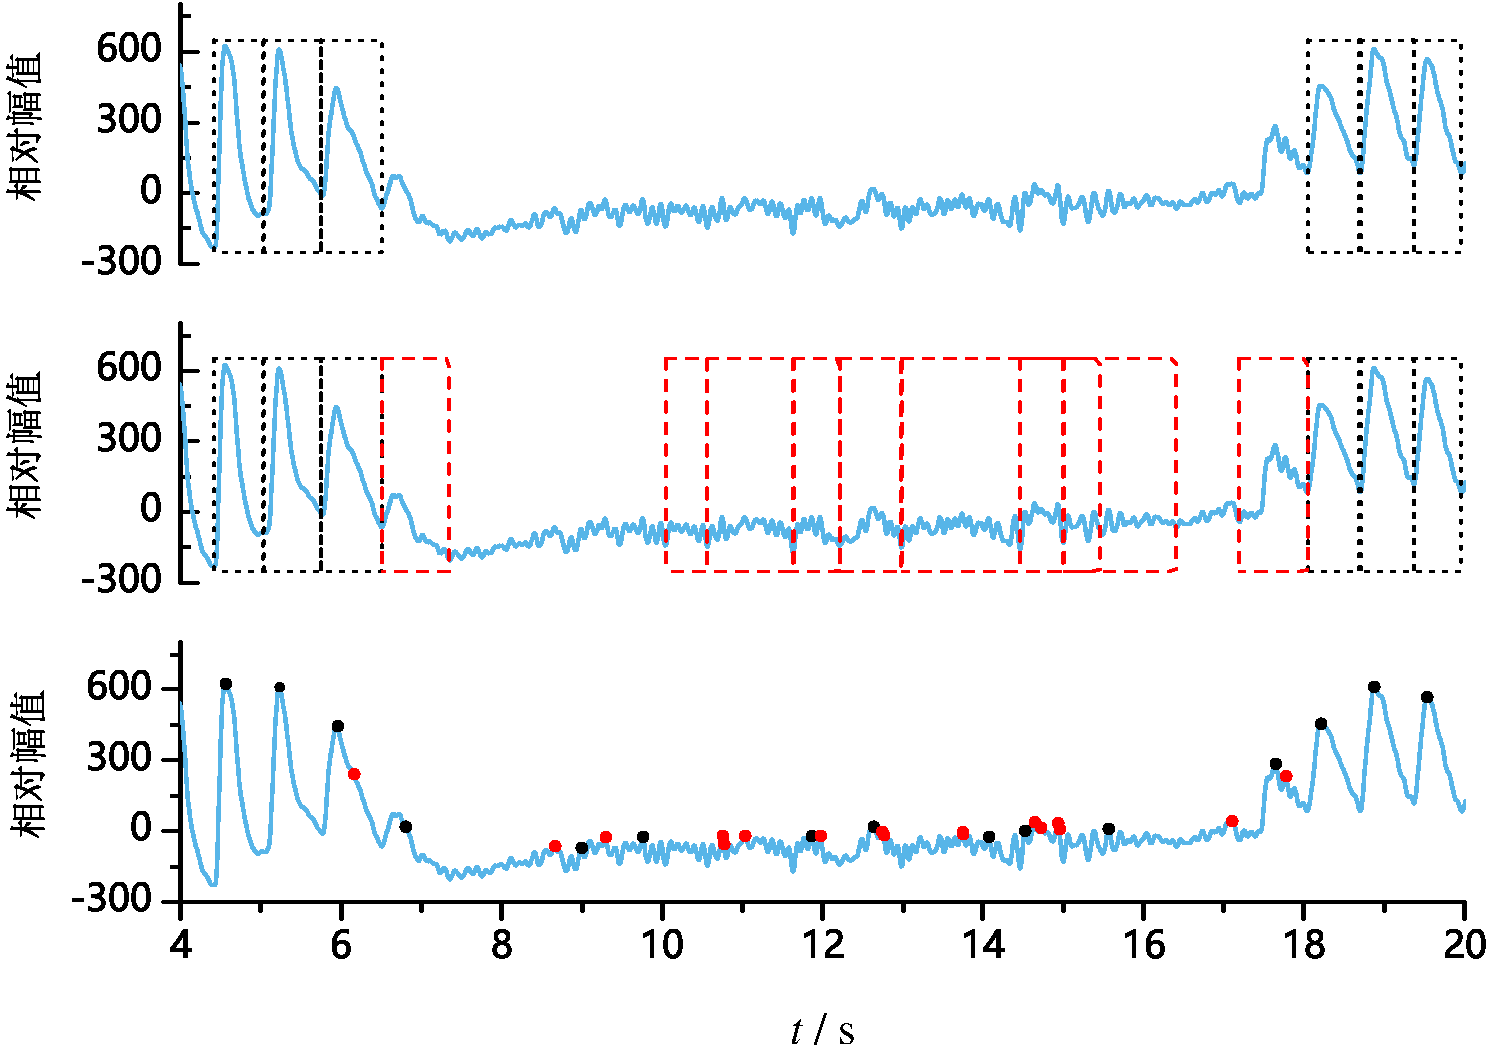
\includegraphics[width=0.9\linewidth]{pulse_preprocess/scd1}
    \caption{\label{fig:scd_detect1}三种PPG检波算法对自主实验数据的检测效果对比图}
\end{figure}

\begin{figure}[htbp]
    \centering
    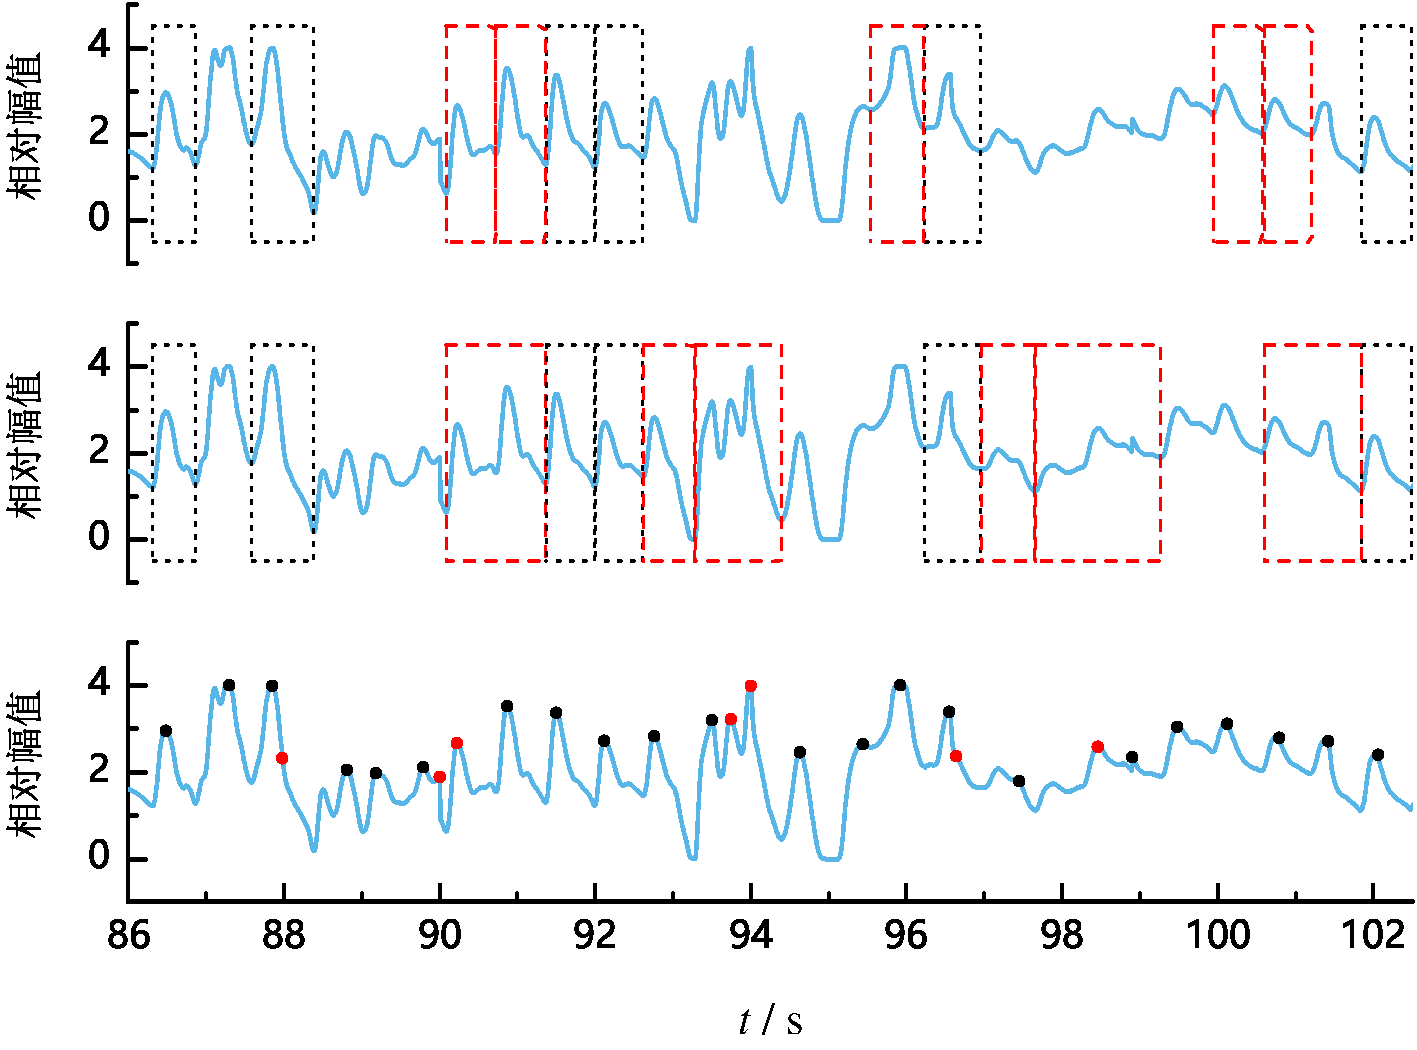
\includegraphics[width=0.9\linewidth]{pulse_preprocess/scd2}
    \caption{\label{fig:scd_detect2}三种PPG检波算法对CBPEDS中数据的检测效果对比图}
\end{figure}
\noindent
数据波形畸变严重,显著异于常人,如\autoref{fig:ucibp_abnormal}所示。
SCD算法可以准确地识别这些异常波形,不进行波形标注。由于如\autoref{fig:ucibp_abnormal}所示的异常数据不在本研究选作算法性能评估的50条数据内,SCD算法的检测结果未能在\autoref{tab:scd}所示的统计值中得以体现。

五、讨论

本研究对PPG波形的检测过程进行了模式设计,提出了一种新型SCD算法,算法由初筛、复核与决策等三部分组成。
在初筛时,通过搜索窗的方法确定波形;在复核时,通过功率、标准差、波峰相对位置与基线漂移程度等PPG形态学特征,区分有效波形与异常干扰
;在决策时,通过加权投票的策略确定PPG波形是否为有效波形。SCD算法可根据使用场景进行二次开发,支持更改初筛算法、增删复核标准与切换决策策略等设置。
经验证,该算法各模块设计合理,与其他算法对比结果表明,对PPG波形的识别准确率高、抗干扰能力强。SCD算法为多平台、多研究应用下的PPG分析检测的不同场景提供了一定的参考。

\begin{figure}[h]
    \centering
    \subfigure[\label{fig:c_0179}畸变信号示意图(一)]{
        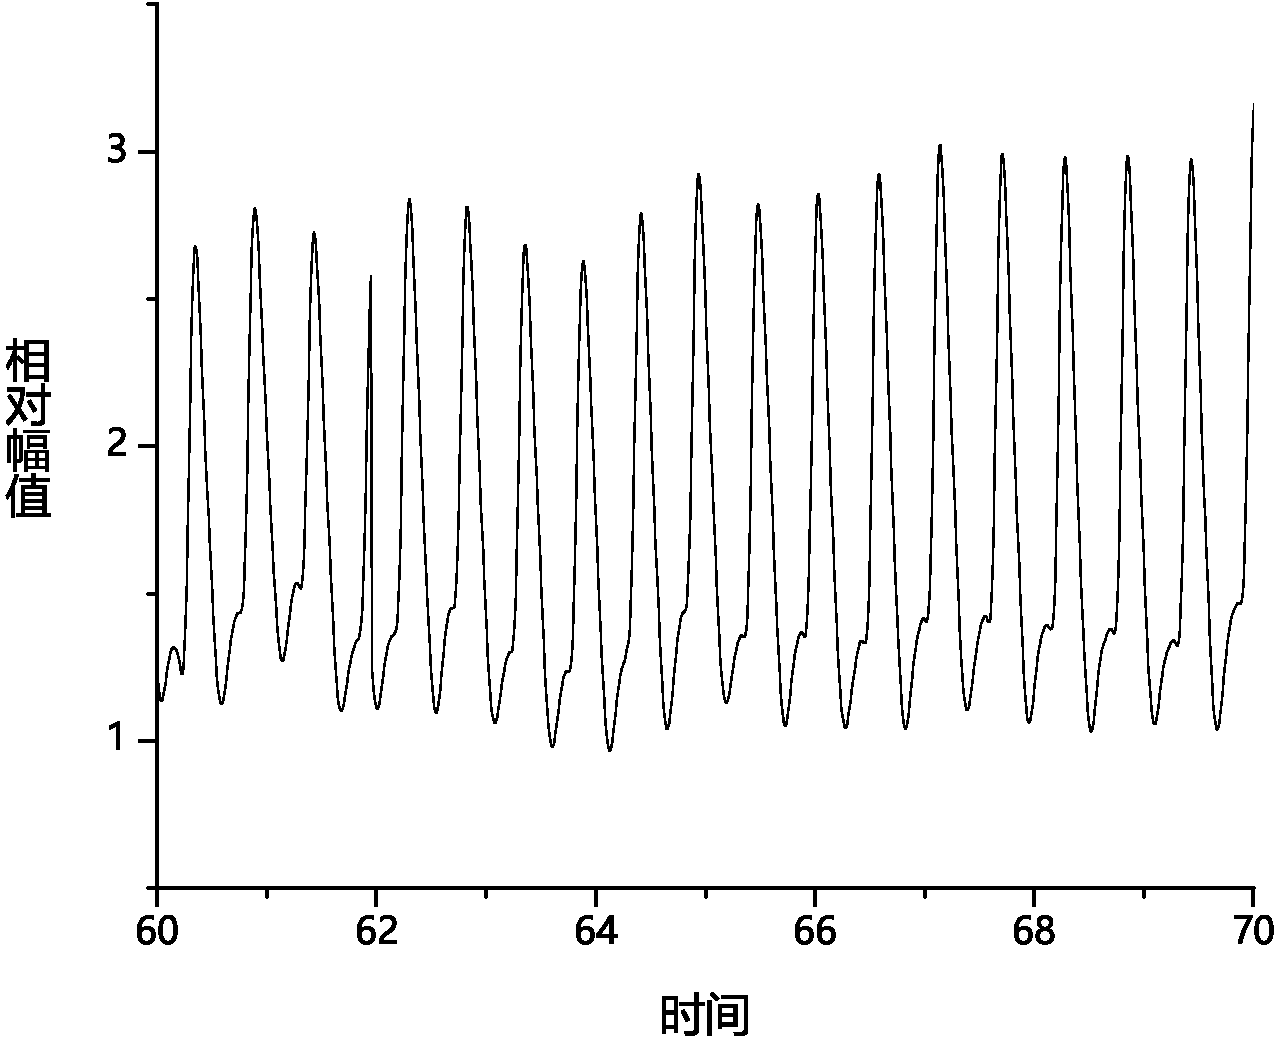
\includegraphics[width=7.5cm]{pulse_preprocess/0179}
    }
    \quad
    \subfigure[\label{fig:c_0533}畸变信号示意图(二)]{
        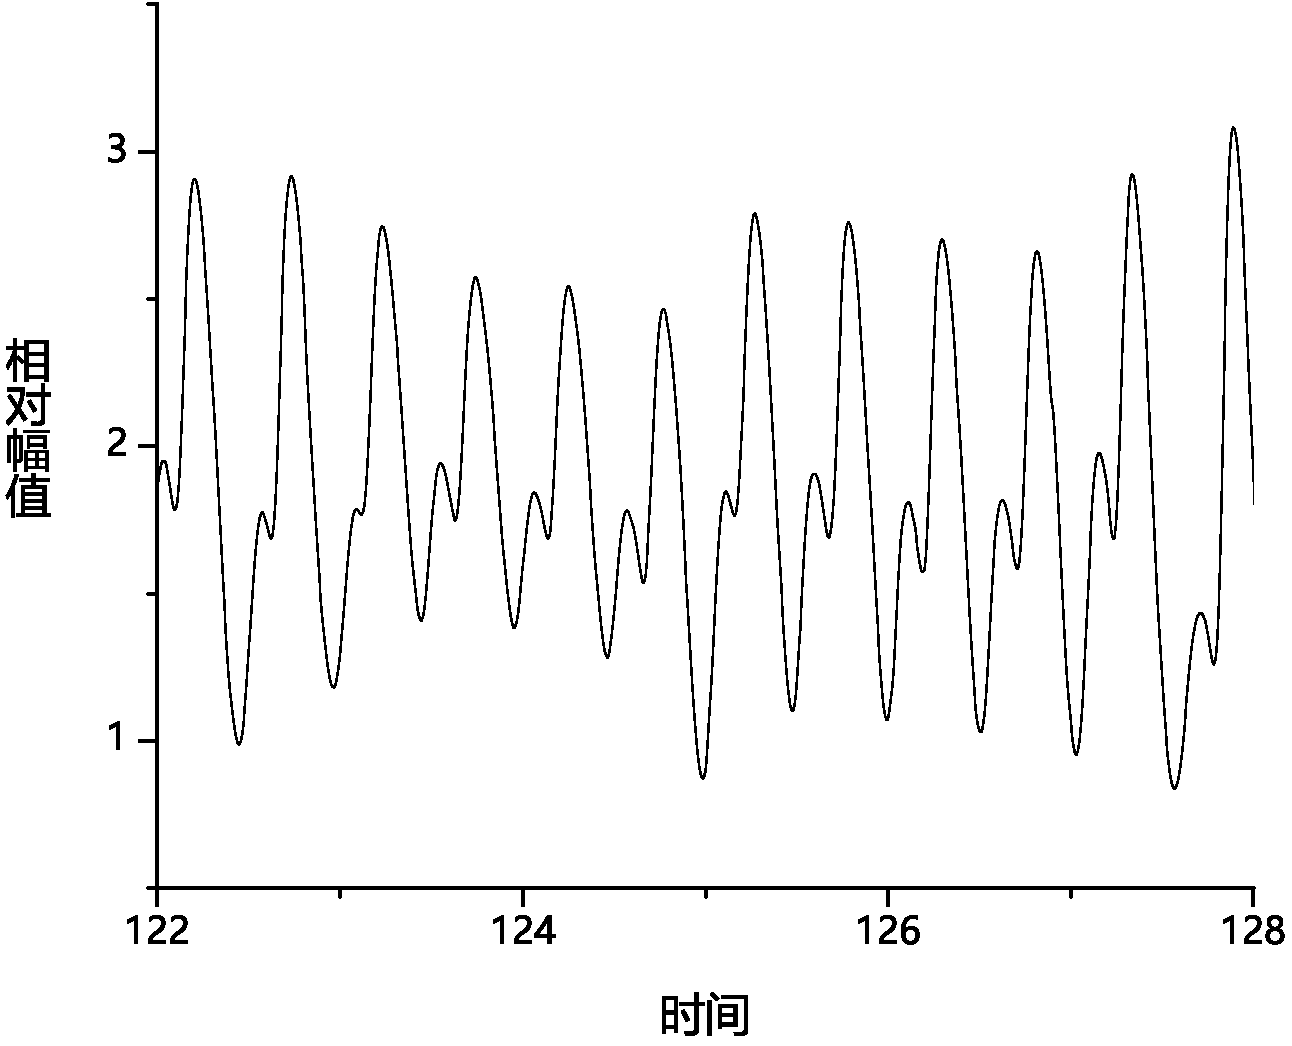
\includegraphics[width=7.5cm]{pulse_preprocess/0533}
    }
    \quad
    \caption{\label{fig:ucibp_abnormal}CBPEDS中畸变信号示意图}
\end{figure}

\subsection{重搏波与切迹检测}
重搏波是PPG最具标志性的波形特征之一,其波峰与切迹的检测是一个完整的PPG检测算法必不可少的定位项之一\cite{Wang2012}。但在实际应用中,并不是每个人的PPG信号都有着明显的重搏波,特别是当被试出现外周阻力增加、血管壁弹性下降的情况后\cite{mmt}。
此时,随着PPG波形向外周传播,尖锐的重搏波切迹(incisura)常会变形甚至丢失,退变成一简单拐点,甚至重搏波波峰都会在下降支中不显著,导致最后无法从采集得到的信号中对两者直接进行精准定位,如\autoref{fig:incisura}所示。

本研究借鉴了王选等\cite{Wang2012}于2012年提出的一种基于曲率$K$(curvature)的定位算法对切迹进行检测,该算法的核心思想是PPG信号在切迹退化成的变形点的邻域内具有最大的曲率值,如\autoref{alg:incisuras_detect}所示。
数学中,将一般曲线函数在点$(x,y)$处的曲率$K$定义为
\begin{equation}
    \label{equ:curvature}
    K=\frac{|y^{''}|}{{(1+{y^{'}}^2)}^{3/2}}
\end{equation}
其中,$y^{'}$与$y^{''}$分别是曲线函数在该点的一阶导数与二阶导数。

\begin{figure}[htbp]
    \centering
    \subfigure[重搏波明显的PPG波形示意图]{
    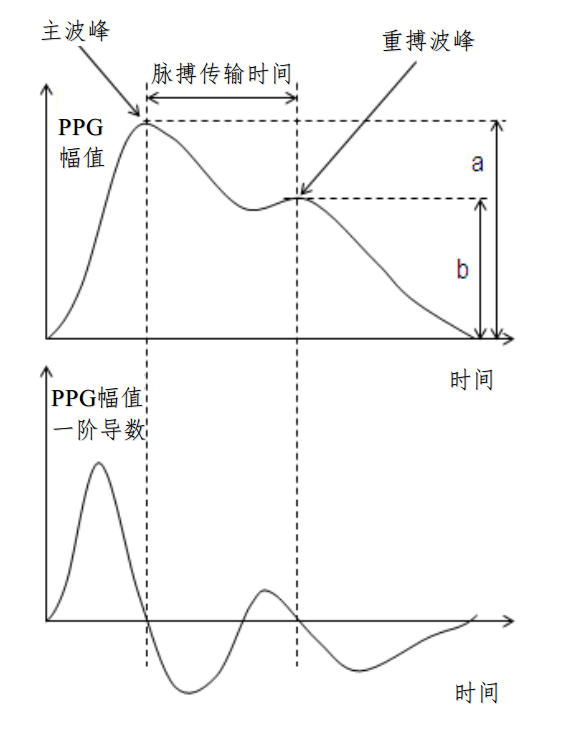
\includegraphics[width=5.5cm]{pulse_preprocess/ri1}
    }
    \quad
    \subfigure[重搏波不明显的PPG波形示意图]{
    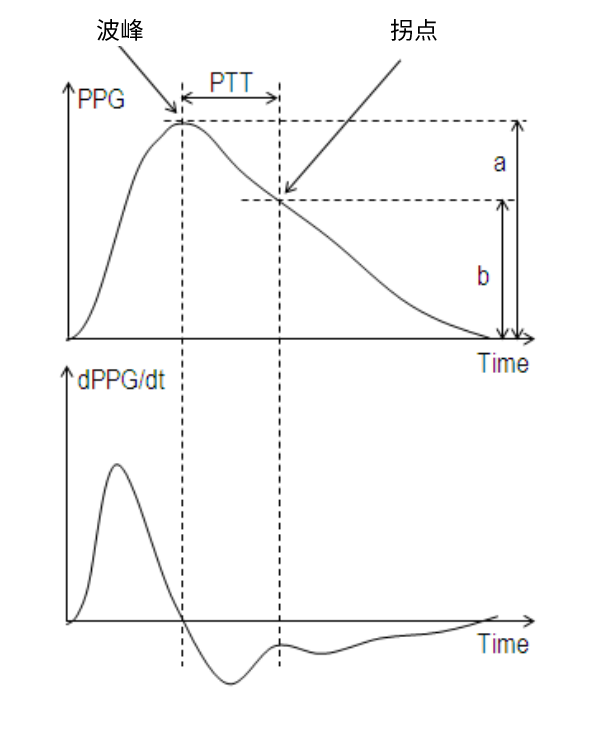
\includegraphics[width=5.5cm]{pulse_preprocess/ri2}
    }
    \caption[重搏波及切迹定位原理示意图]{\label{fig:incisura}重搏波及切迹定位原理示意图\cite{Wang2012,Su2014}}
\end{figure}

\begin{breakablealgorithm}
    \caption{PPG波形切迹定位检测算法}
    \label{alg:incisuras_detect}
    \begin{algorithmic}[1] %每行显示行号
        \Require 原始数据数组$Points$,检测完毕的波形$pulse$,原始数据的一阶差分数组$D$
        \Ensure 当前波形的切迹位置
        \Function {DetectIncisura}{$Points, pulse, D$}
            \State $s \gets pulse.peak.x + \frac{3}{10}(pulse.trough.x-pulse.peak.x)$
            \State $e \gets pulse.peak.x + \frac{9}{10}(pulse.trough.x-pulse.peak.x)$
            \State \Comment 切迹可能出现的位置为波形的下降支中后部分。
            \State $M  \gets \Call{Max}{$D[s],D[e]$}$
            \State \Comment 寻找到上述区间内一阶导数最大值点记为$M$。
            \If{$D[M] >0$}
                \State \Comment 下降支中存在明显的重搏波。
                \State $Incisura \gets \Call{Min}{Points[s],Points[M]}$
                \State \Comment 重搏波波峰即为点M至脉搏波终点之间的极大值点,切迹为脉搏波波峰至点M之间的最小值点。
            \Else
                \State \Comment 下降支一直单调下降,不存在明显的重搏波。
                \State $Incisura \gets \textproc{Min}({\Call{Curvature}{Points[M],Points[e]}})$
                \State \Comment 重搏波波峰定义为点M至脉搏波终点之间的曲率最大处,切迹定义为脉搏波波峰至点M之间的曲率最小处。
            \EndIf
            \State \Return{$Incisuras$}
        \EndFunction
    \end{algorithmic}
\end{breakablealgorithm}

\subsection{信号的重采样}
通常而言,在一项具体的应用研究中,PPG数据的采样率维持不变的。但在某些情况下,原始数据采样率不能满足实际需求,需要进行采样率调整才能满足特定的数值计算需求。
其中,减少抽样率的过程称为信号的抽取,也称抽样率压缩;增加抽样率的过程则称之为信号的插值,也即抽样率扩张\cite{Cheng2008}。信号的抽取与插值都会导致原始信号出现频谱迁移,即改变信号的频率成份\cite{Cheng2008}。

相对而言,信号的抽取过程更容易理解。若需要用整数$D$对$x(n)$进行抽取,以使抽样率降低到原始值的$1/D$,可按照每连贯的$D$个抽样中取出一个信号值。这样的处理称为整数$D$抽取\cite{Cheng2008}。
插值是抽取的逆过程,通过某些已知的数据点去推断一个(系列)特定的函数,使得所有已知数据点均在该函数图像上,从而去推断更多未知数据点,这一过程如\autoref{fig:spline}所示。若不考虑可能出现的信号失真,理论上
可以通过调整抽取与插值的数值对原始信号的采样率进行任意的调整。
\begin{figure}[htbp]
    \centering
    \subfigure[经过点(1,2),(2,1),(4,4)和(5,3)的线性样条示意图]{
    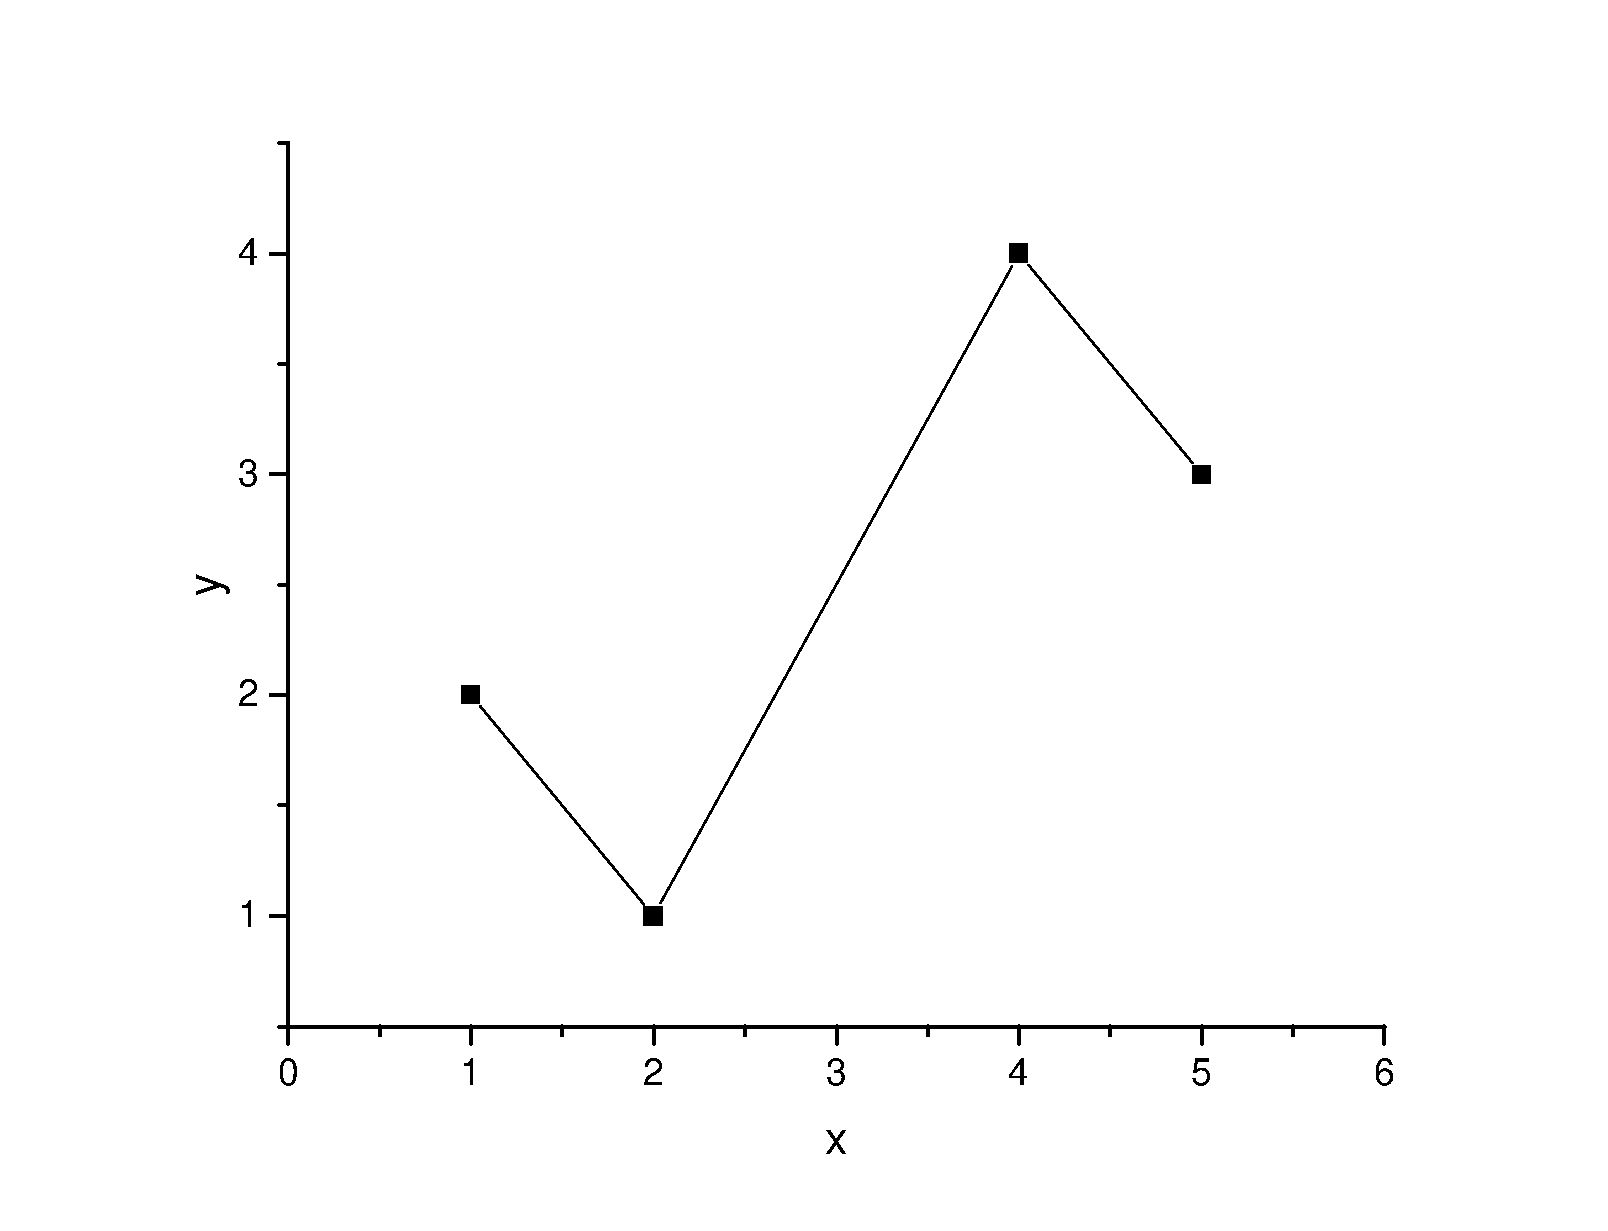
\includegraphics[width=5.5cm]{pulse_preprocess/spline1}
    }
    \quad
    \subfigure[经过相同点的一种可能的三次样条插值示意图]{
    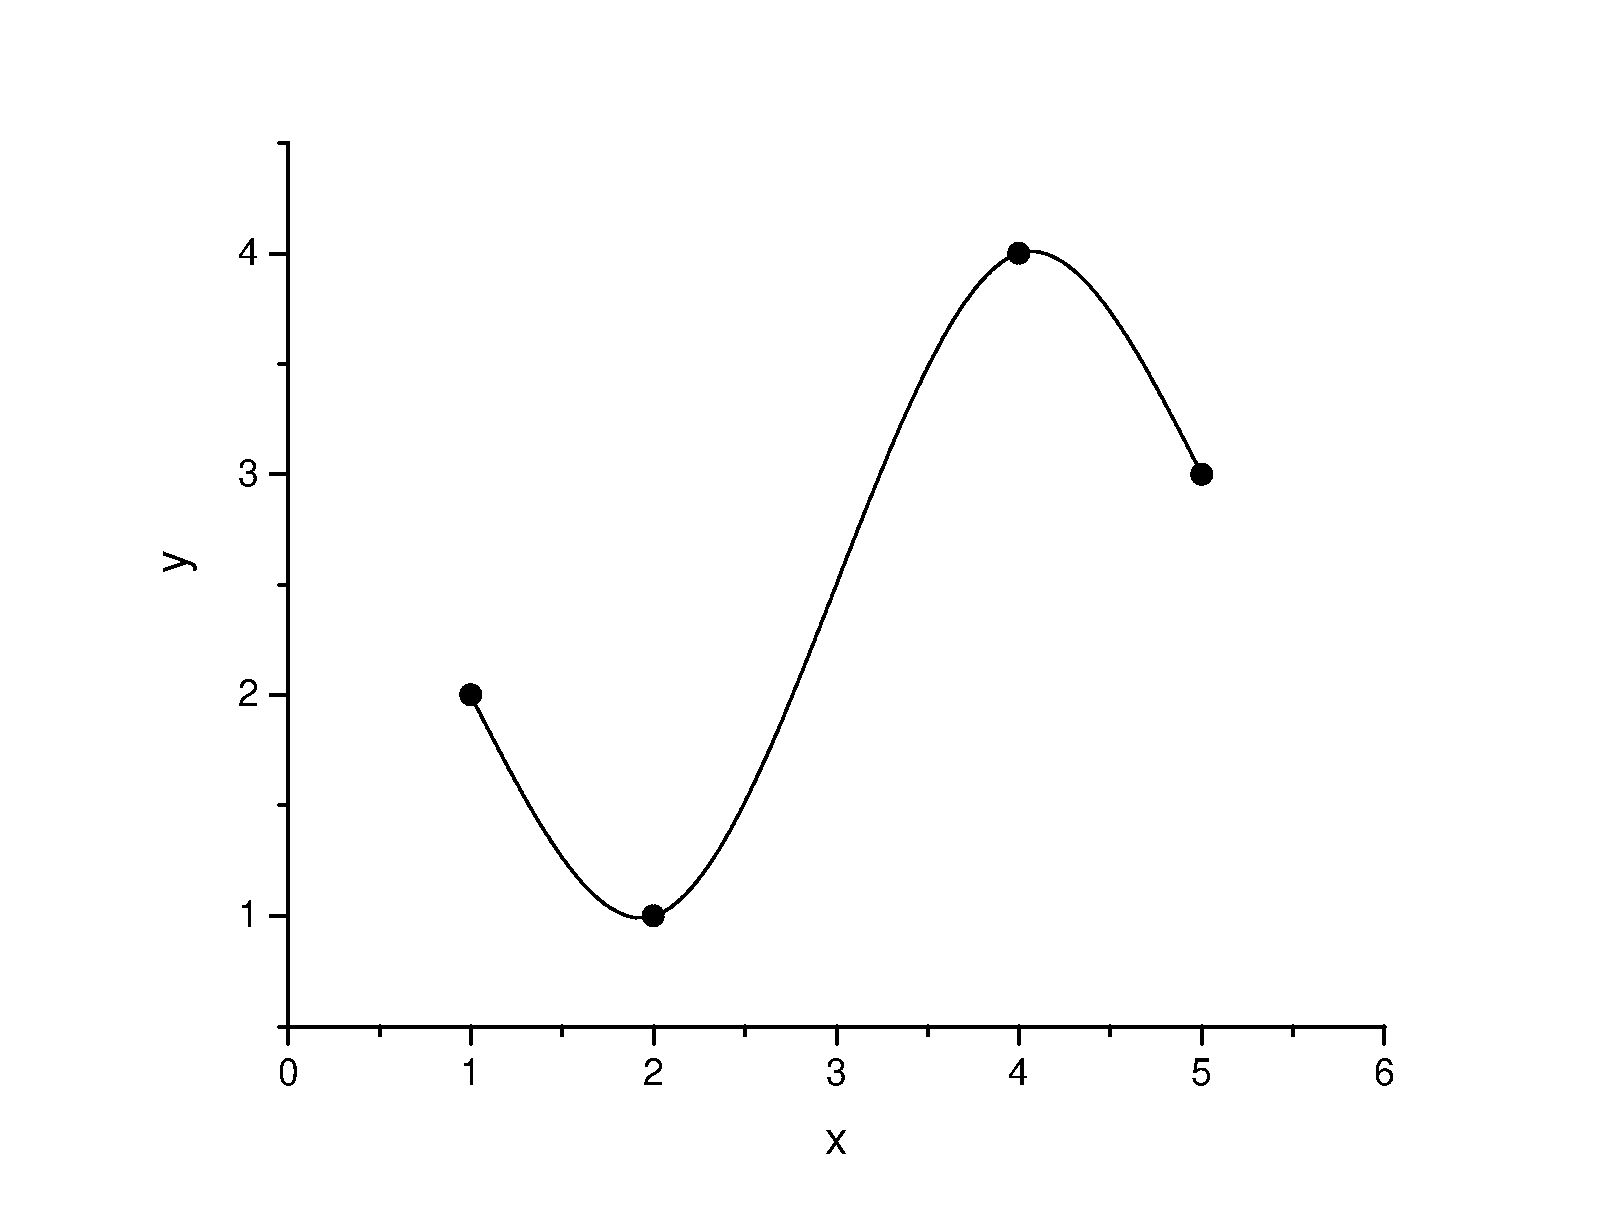
\includegraphics[width=5.5cm]{pulse_preprocess/spline2}
    }
    \caption{\label{fig:spline}两种样条插值方法示意图}
\end{figure}

本论文采用了三次样条插值算法进行插值\cite{Timothy2018,Carl2008}。样条插值是在工业领域应用最广泛的算法之一,它使用多个公式来通过所有数据点并得到得到光滑的拟合插值曲线,
其中每个公式均为低阶多项式。

对原始数据点$(x_1,y_1),(x_1,y_1),\cdots,(x_n,y_n)$,三次样条的插值曲线$S(x)$在每两个数据分段区间$[x_i,x_{i+1}]$内均使用三阶多项式
\begin{equation}
    \label{equ:spline}
    S_{i}=y_{i}+b_{i}(x-x_{i})+c_{i}{(x-x_{i})}^2+d_{i}{(x-x_{i})}^3
\end{equation}
并保证每两个多项式在端点(即原始数据点)处不仅数值相等,相应的斜率与曲率均相等。
仅基于以上条件得到的方程组具有无穷多组解,即可以构造处无穷多条通过所有数据点$(x_i,y_i)$的样条曲线。
为使其存在唯一解,需要添加额外的方程对样条曲线进行约束,一般的约束条件都是对样条左右端点处进行限定。
依据附加边界条件的不同,可进一步将三次样条算法分为自然三次样条、曲率调整三次样条、钳制三次样条、抛物线端点三次样条与非纽结三次样条等\cite{Timothy2018}。

为计算本研究后续章节提出的多种PPG时域特征,本研究使用了基于自然边界条件的三次样条算法对PPG信号进行均匀插值。
3.1节中数据实验所采用的设备GE B450设备的采样率仅为100Hz,重采样处理后的PPG数据采样率被提高至2000Hz。

\subsection{去除基线漂移}
由于呼吸干扰等原因,实际得到的PPG波形的起始点幅值(即连续两个波形的波谷幅值)很难保持一致。这种差异最终会导致PPG信号的基线出现波动漂移,如\autoref{fig:drift}所示。为满足后续特定PPG形态特征计算需求,
需要消除基线漂移的影响。
本研究借助一种基于线性变换的思路完成了基线漂移处理。将一个包含$n$个采样点的PPG波形的幅值表示为序列$x_i$,其中$0 \le i \le n-1$。
由于始末位置脉搏波幅值不等,则明显两者之间存在一条斜率$k \ne 0$的直线,其中
\begin{equation}
    \label{equ:linek}
    k=\frac{x_0-x_{n-1}}{n-1}
\end{equation}
则该直线上任意点即代表了在该时刻PPG波形与水平基线的偏移量,即
\begin{equation}
    \label{equ:liney}
    \Delta_i=ki+x_0
\end{equation}
此时,去除基线漂移后的PPG信号可标示为
\begin{equation}
    \label{equ:adjusta}
    y_i=x_i-\Delta_i
\end{equation}

\begin{figure}[htbp]
    \centering
    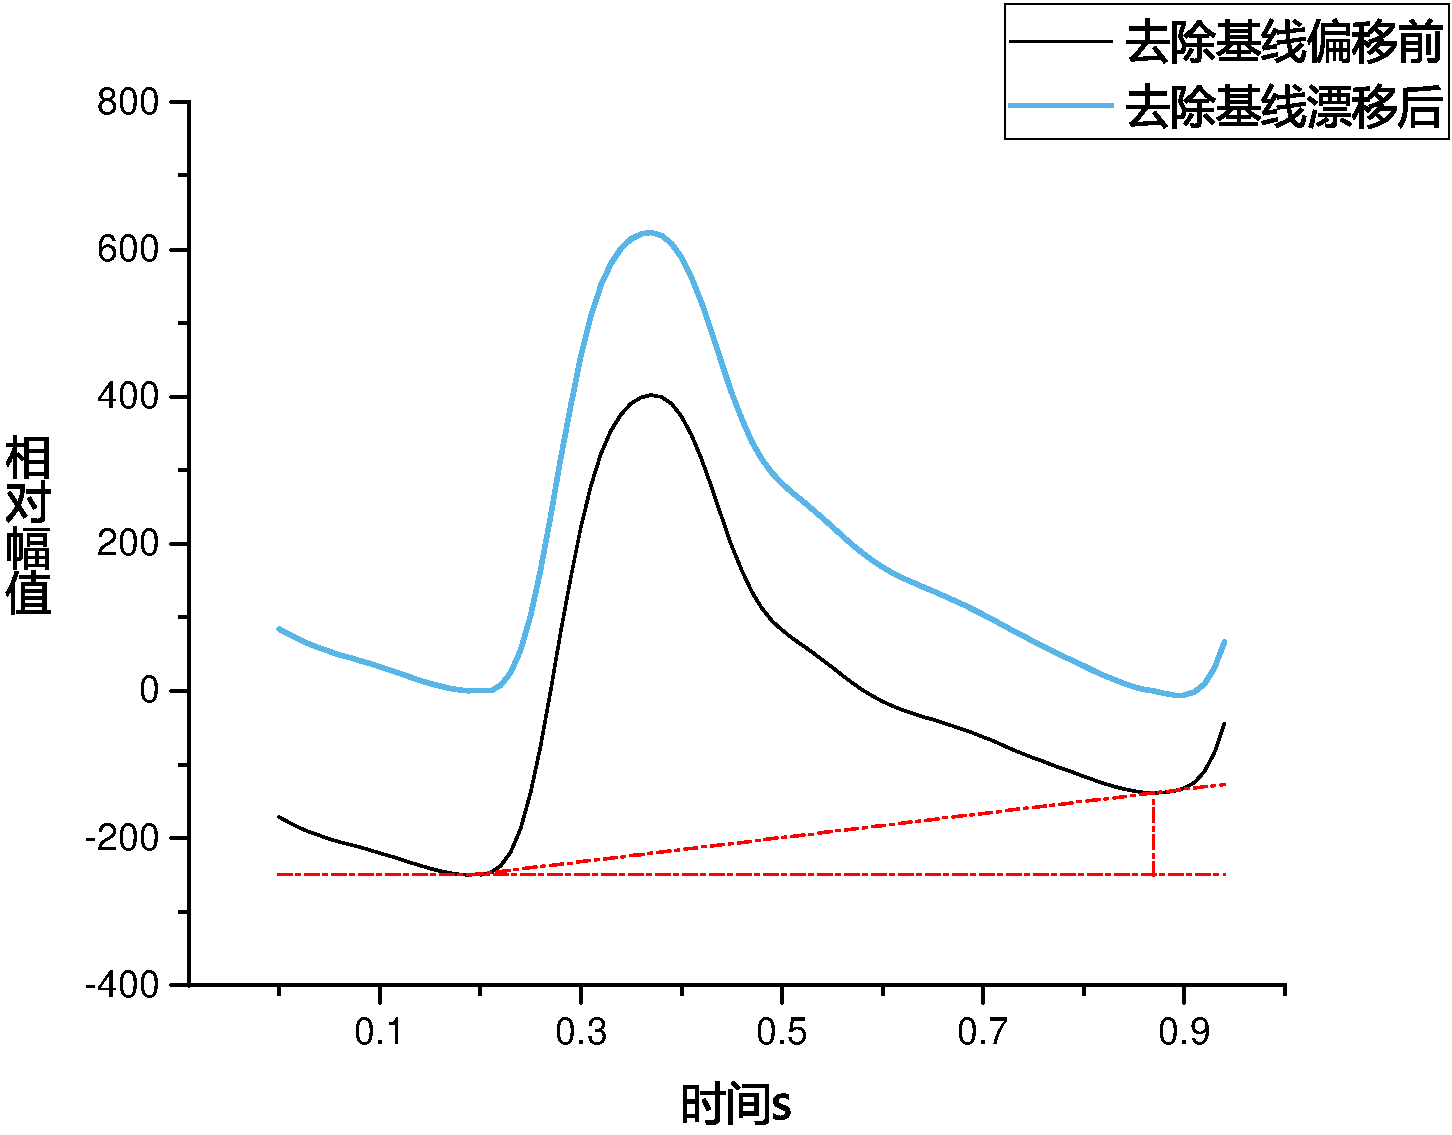
\includegraphics[width=.6\linewidth]{pulse_preprocess/baselineadjust}
    \caption{\label{fig:drift}基线漂移去除原理示意图}
\end{figure}

\subsection{数据标准化}
在上述各项预处理过程完成后,PPG波形在幅值上仍然有很大的个体差异,即使对同一被试对象,其波形在幅值上也会有一定的波动,如\autoref{fig:pulses_of_person}所示。为消除个体差异对特定波形特征计算的影响,需要对PPG波形进行归一化处理。
\begin{figure}[htbp]
    \centering
    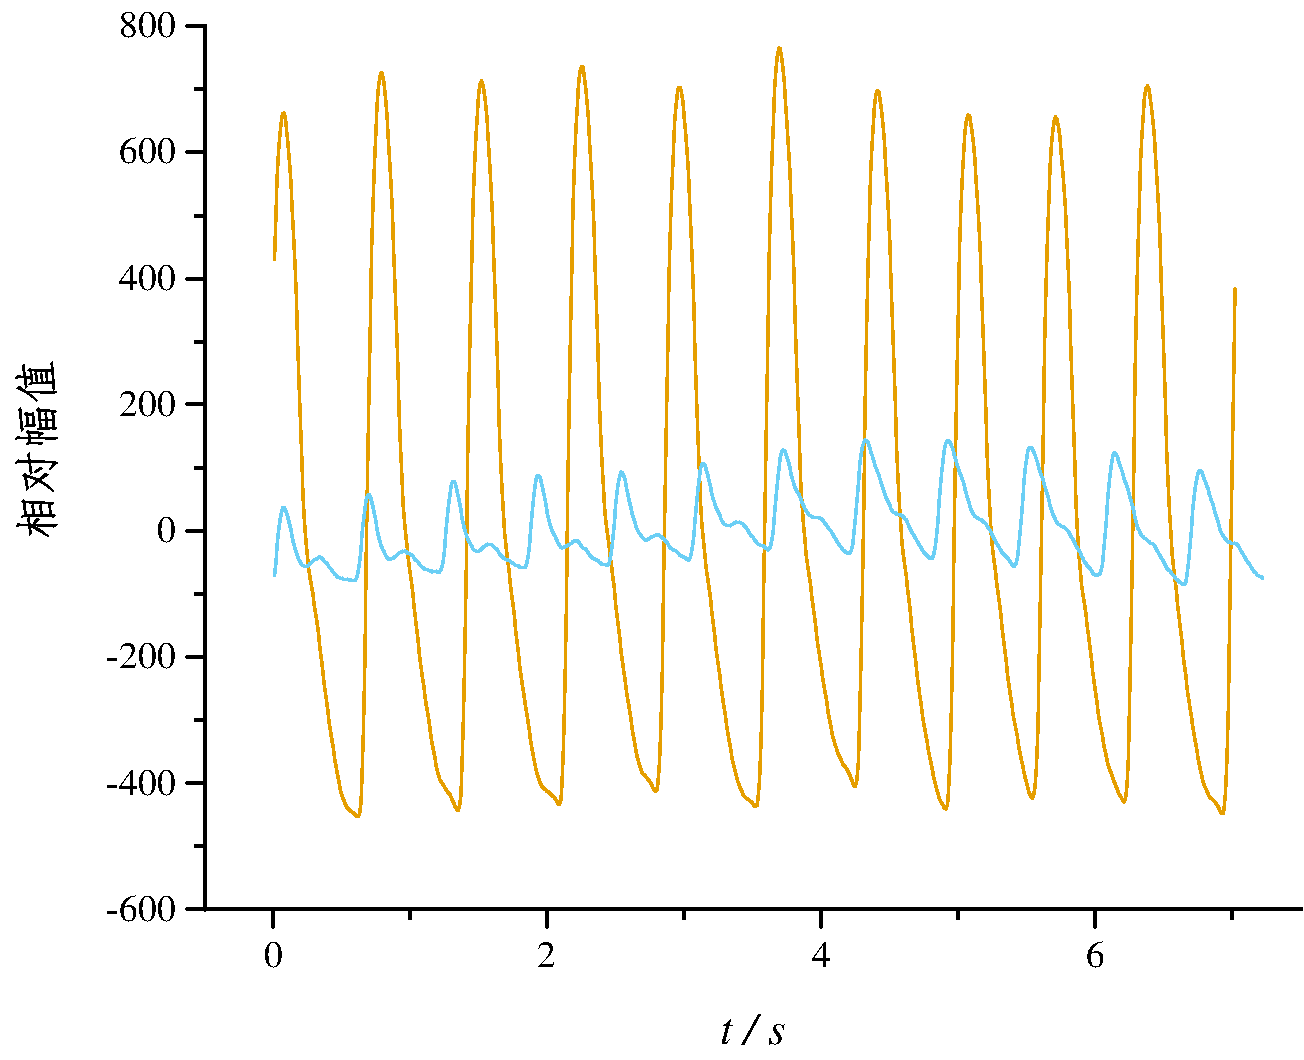
\includegraphics[width=.6\linewidth]{pulse_preprocess/pulses_of_person}
    \caption{\label{fig:pulses_of_person}临床实验采集得到的不同个体的PPG波形幅值对比图}
\end{figure}

时间标准化与幅值标准化是PPG标准化两类常见的方式\cite{mmt}。时间标准化的基本原理是将PPG信号进行分组并计算每组信号的平均心动周期,随后对每组内的PPG信号进行时间尺度上的缩放,使最终的总平均心动周期保持一致。
由于不同个体的时间尺度上的缩放比例不一致,很容易导致PPG信号波形发生畸变失真,严重影响后续特征计算。
第二章已经介绍过,PPG本身是人体指端血液容积变化率的体现,且由于人体指端血液容积因人而异,故PPG信号的波形幅值对不同个体而言并无实际的生理意义。因此,本研究采取了幅值标准化的处理方式对PPG信号进行处理。

与去除基线漂移过程类似,为使幅值标准化,只需对PPG波形内所有采样点进行一次线性变换
,使单个波形内所有数据点按同一尺度缩放映射到[0,1]区间内。
所有波形的标准化系数即缩放比例也同时被保存记录下来。

\section{脉搏波的时域特征}
PPG信号本身蕴含着丰富的血液动力学信息,其形态、强度、速率、节律等特征可以反映心脏的功能与状态,也可以反映出各级动脉及分支中血管壁弹性、血管阻力、血液黏度等信息,是评价人体心血管系统生理病理状态的重要依据\cite{PPGYY}。
这也就是说,PPG信号携带了能够表征人体心血管系统生理病理状态的丰富信息,这些信息蕴藏在了PPG波形的变化之中。因此,用何种方式描述、获取、挖掘这些信息,是基于脉搏波的分析工作能够开展的前置条件。

在PPG波形的诸多特征参数中,包括时间类参数、幅度类参数、面积类参数与斜率类参数在内的时域特征参数往往定义清晰明了、意义明确易于理解,易与脉搏波产生原理过程联系起来,可解释性强。
因此,这些参数在基于PPG的各类研究中得到了最广泛的应用\cite{cwl,mmt}。本节对此类时域特征进行汇总整理介绍,特别地,本节也对已在PE研究中得到应用的PPG进行说明。

\subsection{时间类特征参数}
时间类特征参数描述了PPG波形中某些特殊点之间的时长或多个时长之间的比例关系。其中,脉搏传导时间(pulse transit time,PTT)是最有代表性的时间类参数之一\cite{Brumfield2005,Su2014}。
如\autoref{fig:ri}所示,PTT是对脉搏波主波峰与重搏波波峰或反射波导致的拐点之间的时间间隔的量化描述。
\begin{figure}[htbp]
    \centering
    \subfigure[\label{fig:ri1}重搏波明显的PPG波形示意图]{
    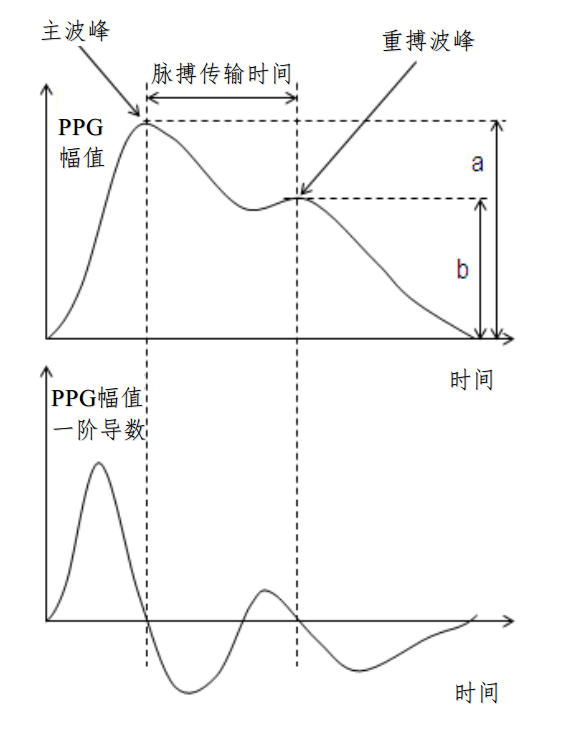
\includegraphics[width=6cm]{pulse_preprocess/ri1}
    }
    \quad
    \subfigure[\label{fig:ri2}重搏波不明显的PPG波形示意图]{
    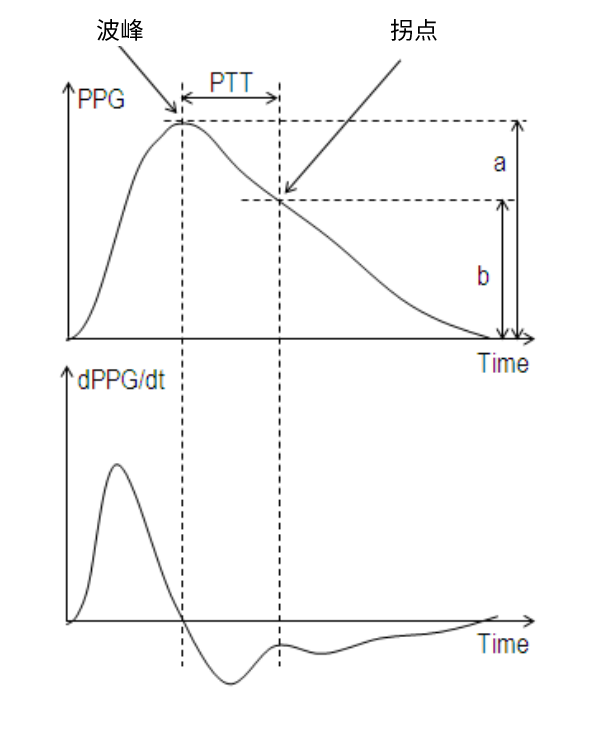
\includegraphics[width=6cm]{pulse_preprocess/ri2}
    }
    \caption[PTT及RI计算原理示意图]{\label{fig:ri}PTT及RI计算原理示意图\cite{Su2014}}
\end{figure}

除PTT外,时间类特征参数还包含脉搏波脉动周期、上升支间期、下降支间期等。2016年,王梦婷\cite{mmt}提出了一种描述动脉内高压力水平维持的时间参数,并在此基础上归一化处理后得到了多项衍生参数,
包含动脉高压力持续时间、血管硬度指数、心肌收缩系数及心博出系数等。
2018年,陈婉琳等\cite{cwl}基于斜率极值提出了上升支最大斜率间期、下降支最小斜率间期等参数。
\begin{figure}[htbp]
    \centering
    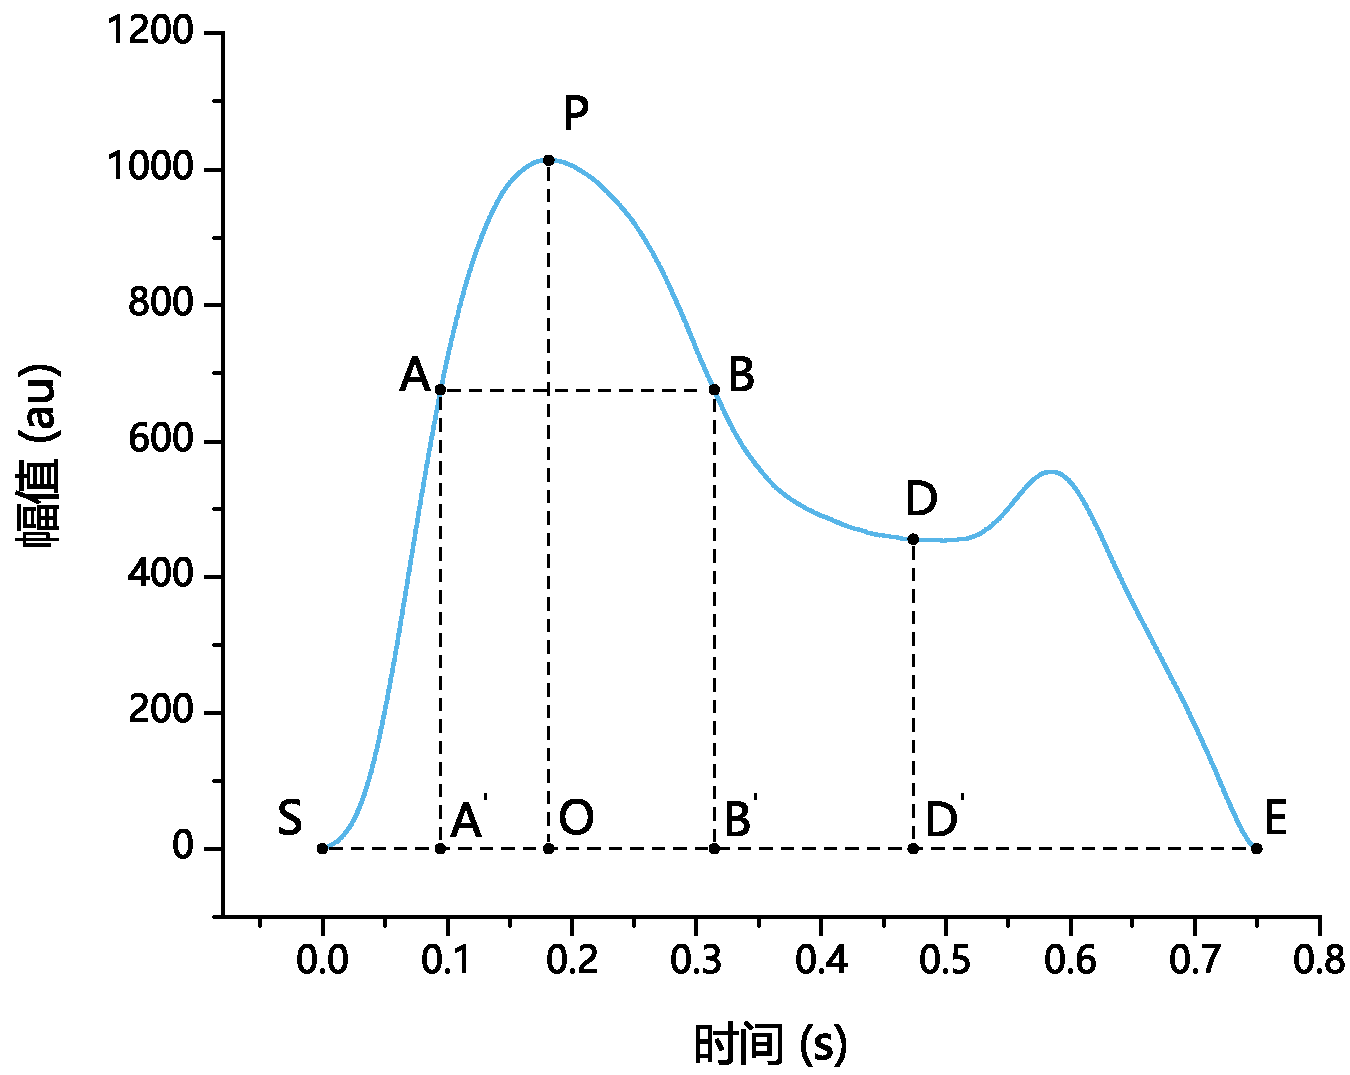
\includegraphics[width=.55\linewidth]{pulse_preprocess/timefeature}
    \caption[常见的PPG时间及幅值类参数示意图]{\label{fig:timefeature}PPG时间及幅值类参数示意图}
\end{figure}

以上参数的定义参见\autoref{fig:timefeature}及\autoref{tab:timefeature}所示,
\autoref{fig:timefeature}中$AA'$的幅值为主波峰值的2/3,$D$点为降中峡\cite{mmt};\autoref{tab:timefeature}则给出了各特征的定义及在\autoref{fig:timefeature}中的对应表达式。

\begin{longtblr}
    [
        theme          = {zju},
        caption        = {常见的PPG时间类参数},
        label          = {tab:timefeature},
    ]
    {
        colspec        = {X[1,c,m]X[4,c,m]X[8,c,m]X[2,c,m]},
        hline{1,Z}     = {\thickline},
        hline{2}       = {\thinline},
        rowhead        = 1,
        row{1}         = {font=\headfont},
        row{2-Z}       = {font=\nonheadfont},
    }
    序号 & 参数 & 物理意义 & 表达式 \\
    1 & 脉动周期      &  相邻两个波谷之间的时间间隔         &  $SE$\\
    2 & 上升支间期      &  从波形起点(波谷)至主波峰之间的时间间隔         &  $SO$\\
    3 & 下降支间期      &  从主波峰至波形终点(波谷)之间的时间间隔        &  $OE$\\
    4 & 动脉高压力持续时间    &  主波维持在峰值幅值2/3高度的时间间隔         &    $A'B'$   \\
    5 & 血管硬度指数    &  动脉高压力持续时间与脉动周期的比值         &   $\displaystyle \frac{A'B'}{SE}$    \\
    6 & 心肌收缩系数    &  上升支间期与脉动周期的比值         &  $\displaystyle \frac{SO}{SE}$    \\
    7 & 心搏出系数      &   从波峰至降中峡的时间间隔与脉动周期的比值       &   $\displaystyle \frac{OB'}{SE}$\\
    8 & 上升支最大斜率间期      &   上升支波谷与上升支斜率最大点之间的时间间隔      &   /    \\
    9 & 下降支最大斜率间期      &   下降支斜率最小点与下降支波谷之间的时间间隔      &    /  \\
\end{longtblr}

\subsection{幅值类特征参数}

幅值类特征参数描述了PPG波形中某个时刻的幅值高度或多个幅值高度之间的比例关系。
在研究不同个体间的PPG波形相关问题时,绝对值类的幅值特征参数由于没有实际的生理意义不具可比性,但幅值相关的比值与变化率类的特征参数仍能在此类研究中发挥重要作用,
包括脉搏波增强指数(augmentation index,AIX)、反射指数(reflection index,RI)及K值等\cite{Su2014,Elgendi2012,Luo1988,PPGYY}。

AIX指心脏收缩期早期与晚期拐点之间的差值与峰值之比,计算的关键需要先找到表征脉搏波反射波上升冲程(up-stroke)的拐点$P_1$,如\autoref{fig:aix}所示\cite{Su2014}。
\begin{equation}
    \label{equ:aix}
    \text{AIX} = \pm \frac{\Delta P}{PP}
\end{equation}

特别地,\autoref{equ:character}中$\pm$的取值视拐点$P_1$与峰值点的相对位置而定,当拐点在脉搏波波峰点左侧时,AIX符号取正,表示主波峰是经过叠加“增强”得到的,如图\autoref{fig:aix1}所示;反之,
当拐点在脉搏波波峰点右侧时,AIX符号取负,表明主波峰未得到“增强”,如图\autoref{fig:aix2}所示。
\begin{figure}[htbp]
    \centering
    \subfigure[\label{fig:aix1}拐点在PPG波峰左侧示意图]{
    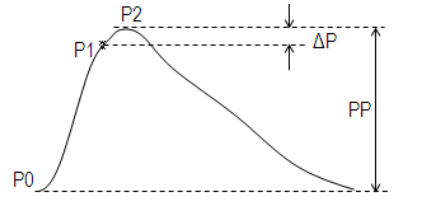
\includegraphics[width=6cm]{pulse_preprocess/aix1}
    }
    \quad
    \subfigure[\label{fig:aix2}拐点在PPG波峰右侧示意图]{
    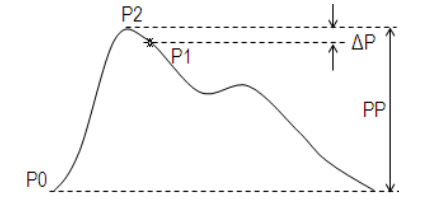
\includegraphics[width=6cm]{pulse_preprocess/aix2}
    }
    \caption[AIX计算原理示意图]{\label{fig:aix}AIX计算原理示意图\cite{Su2014}}
\end{figure}

RI是由脉搏波舒张峰值或拐点处幅值与收缩谷值之比计算得到的,如\autoref{fig:ri}所示\cite{Su2014,Elgendi2012}
\begin{equation}
    \label{equ:ri}
    \text{RI} = \frac{b}{a} \cdot 100\%
\end{equation}

K值是另一种在临床得到广泛应用的基于脉搏波面积变化的形态学特征无量纲参数,最早由罗志昌等\cite{Luo1988,PPGYY}提出
\begin{equation}
    \label{equ:ppgk}
    K=\frac{P_m-P_d}{P_s-P_d}
\end{equation}
其中,$P_m=\frac{1}{T}\int_{0}^{T}P(t)dt$为一个心动周期内脉搏压力$P(t)$的平均值,$P_s$与$P_d$分别为收缩压与舒张压,如\autoref{fig:k}所示。
罗志昌等\cite{Luo1988,PPGYY}的研究表明,K值依赖于脉搏波的波形动态变化,
同时能够在很大程度上反应血管外周阻力与血管壁硬化程度等生理因素的变化。
\begin{figure}[htbp]
    \centering
    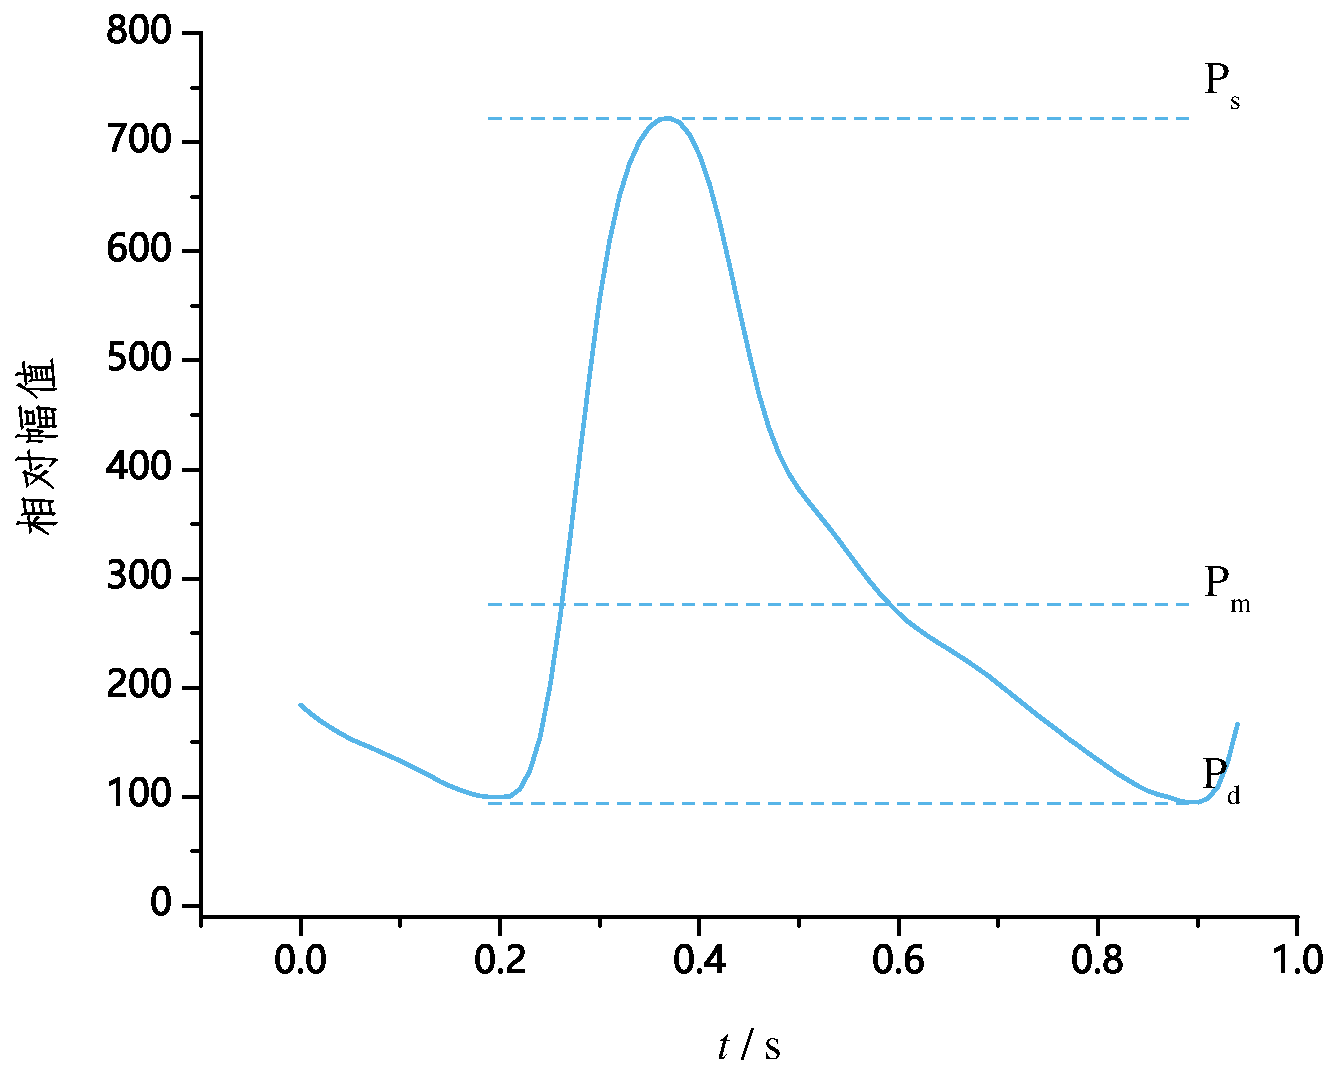
\includegraphics[width=.55\linewidth]{pulse_preprocess/k}
    \caption{\label{fig:k}K值计算原理示意图}
\end{figure}

除上述参数外,幅值类特征参数还包括脉搏波波峰幅值、波谷幅值差值、降中峡幅值及外周阻力系数等,它们往往作为上述比值、变化率类幅值特征参数的中间计算变量,
常用于对同一个体的PPG形态的研究中\cite{cwl,mmt}。这些参数的具体定义参见\autoref{tab:heightfeature}及\autoref{fig:timefeature}所示。

\begin{longtblr}
    [
        theme          = {zju},
        caption        = {常见的PPG幅值类参数},
        label          = {tab:heightfeature},
    ]
    {
        colspec        = {X[1,c,m]X[4,c,m]X[8,c,m]X[2,c,m]},
        hline{1,Z}     = {\thickline},
        hline{2}       = {\thinline},
        rowhead        = 1,
        row{1}         = {font=\headfont},
        row{2-Z}       = {font=\nonheadfont},
    }
    序号 & 参数 & 物理意义 & 表达式 \\
    1 & 波峰幅值      &  主波峰幅值         &  $OP$\\
    2 & 波谷幅值差值      &  相邻波谷之间的幅值之差         &  /\\
    3 & 降中峡幅值      &  降中峡至基线幅值         &  $DD'$\\
    4 & 外周阻力系数      &  降中峡幅值与主波峰幅值之比         &  $\displaystyle \frac{DD'}{OP}$\\
\end{longtblr}

\subsection{面积类特征参数}

面积类参数计算依赖与脉搏波波形与基线所形成的面积,主要通过按时间方向对PPG波形曲线积分完成计算。
面积类参数可以看成是血管在一段时间内的血液容积的映射。
王梦婷\cite{mmt}在其研究中指出,PPG上升支主要受心脏射血量与血压脉动影响,下降支主要受外周阻力影响。其中,上升支随心脏射血量增加愈益陡峭,射血时间越短,
其形态图像越向左上方凸出;而当外周阻力增加时,会导致动脉血管壁弹性下降,下降支波形向上方凸出。

常见的面积类特征参数包括上升支面积、下降支面积、
全周期面积、上升支面积比、下降支面积比、全周期面积比及下降支面积差值比(area difference ratio,ADR)\cite{Feng2018}等。
值得一提的是,Feng等\cite{Feng2018}已经将ADR应用于PE的研究中,其研究结果显示患有PE的孕妇与正常孕妇在PPG信号的ADR参数上具有统计意义上的显著差异(0.752 VS 0.723,$p$<0.01)。
以上参数的具体定义参见\autoref{fig:areafeature}及\autoref{tab:areafeature}。

\begin{longtblr}
    [
        theme          = {zju},
        caption        = {常见的PPG面积类参数},
        label          = {tab:areafeature},
    ]
    {
        colspec        = {X[1,c,m]X[3,c,m]X[6.5,c,m]X[4.5,c,m]},
        hline{1,Z}     = {\thickline},
        hline{2}       = {\thinline},
        rowhead        = 1,
        row{1}         = {font=\headfont},
        row{2-Z}       = {font=\nonheadfont},
    }
    序号 & 参数 & 物理意义 & 表达式 \\
    1 & 上升支面积      &  从波形起点至峰值点对波形曲线积分所得面积         &  $\displaystyle S_r=\int_{T_S}^{T_P}P(t)dt$\\
    2 & 下降支面积      &  从波形峰值点至终点对波形曲线积分所得面积         &  $\displaystyle S_f=\int_{T_P}^{T_E}P(t)dt$\\
    3 & 全周期面积      &  脉搏波波形在一个完整周期内的积分所得面积         &  $\displaystyle S_t=\int_{T_S}^{T_E}P(t)dt$\\
    4 & 上升支面积比    &  上升支面积与$\triangle OPS$面积之比         &   $\displaystyle R_r=\frac{S_r}{S_{\triangle OPS}}$    \\
    5 & 下降支面积比    &  下降支面积与$\triangle OPE$面积之比        &   $\displaystyle R_f=\frac{S_f}{S_{\triangle OPE}}$    \\
    6 & 全周期面积比    &  全周期面积与$\triangle SPE$面积之比         &   $\displaystyle R_t=\frac{S_t}{S_{\triangle SPE}}$    \\
    7 & 下降支面积差值比 & {下降支面积和$\triangle OPE$面积之差\\ 与$\triangle OPE$面积之比}      &    $\displaystyle \Delta R_f=\frac{S_{\triangle OPE}-S_f}{S_{\triangle OPE}}=1-R_f$\\
\end{longtblr}

\begin{figure}[htbp]
    \centering
    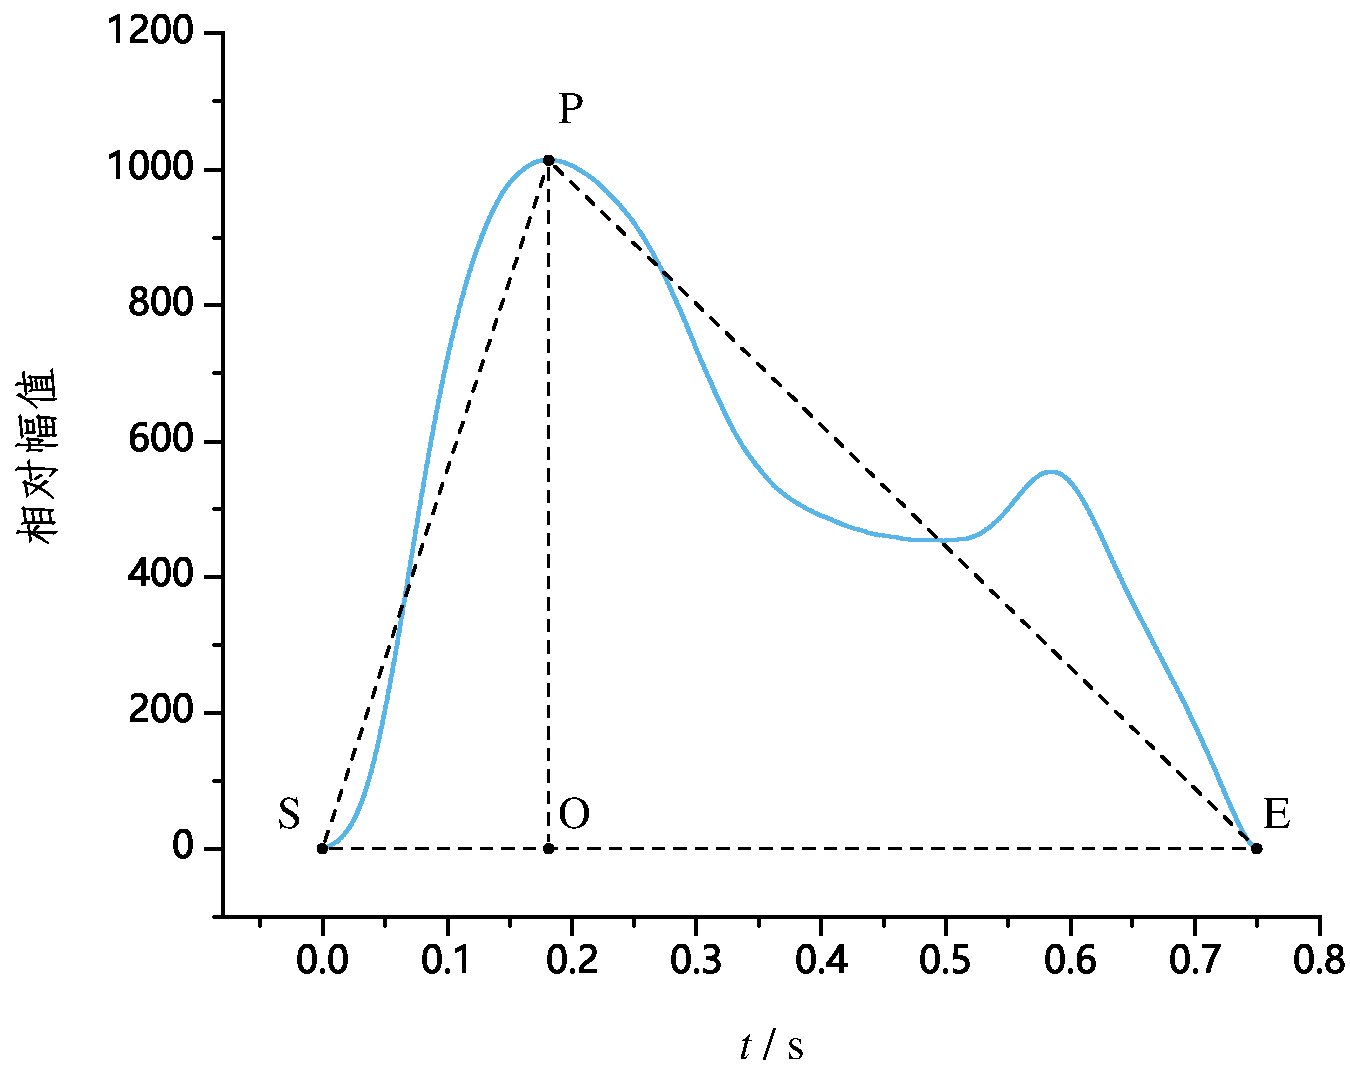
\includegraphics[width=.55\linewidth]{pulse_preprocess/areafeature}
    \caption{\label{fig:areafeature}常见的PPG面积及斜率类参数示意图}
\end{figure}

\subsection{斜率类特征参数}

斜率类参数是对PPG波形在一段时间内幅值的上升或下降速率的量化描述,反应了血液容积在这段时间内的平均流速。

陈婉琳等\cite{Chen2019}提出的光电容积斜率指数(photoplethysmography slope index,PSI)是斜率类参数中比较有代表性的一种,其计算的基本思想是将PPG波形分段后再描述各段之间的幅值变化,
如\autoref{fig:psi}所示。同时,陈婉琳等研究发现PSI可以在一定程度上对PE患者进行识别\cite{Chen2019}。
\begin{figure}[htbp]
    \centering
    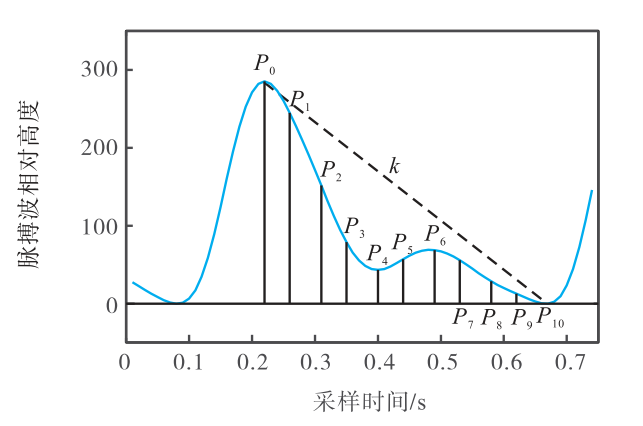
\includegraphics[width=.7\linewidth]{pulse_preprocess/psi}
    \caption[PSI计算原理示意图]{\label{fig:psi}PSI计算原理示意图\cite{Chen2019}}
\end{figure}

此外,常见的斜率参数还包括上升支平均斜率、上升支最大斜率、下降支平均斜率、下降支最大斜率等。这些参数的具体定义参见\autoref{fig:areafeature}及\autoref{tab:slopefeature}所示。
\begin{longtblr}
    [
        theme          = {zju},
        caption        = {常见的PPG斜率类参数},
        label          = {tab:slopefeature},
    ]
    {
        colspec        = {X[1,c,m]X[4,c,m]X[8,c,m]X[2,c,m]},
        hline{1,Z}     = {\thickline},
        hline{2}       = {\thinline},
        rowhead        = 1,
        row{1}         = {font=\headfont},
        row{2-Z}       = {font=\nonheadfont},
    }
    序号 & 参数 & 物理意义 & 表达式 \\
    1 & 上升支平均斜率      &  主波峰值与上升支时间之比         &  $\displaystyle \frac{OP}{SO}$\\
    2 & 下降支平均斜率      &  主波峰值与下降支时间之比         &  $\displaystyle -\frac{OP}{OE}$\\
    3 & 上升支最大斜率      &  上升支一阶导数的最大值        &  /\\
    4 & 下降支最小斜率      &  下升支一阶导数的最小值         &   /    \\
\end{longtblr}

\subsection{其他特征}

除上述特征参数外,在其他研究领域,PPG也有一些较为知名的特征参数,大动脉僵硬指数(stiffness index,SI)与脉搏波波形速度(pulse wave velocity,PWV)就是其中最为典型的代表。

SI被定义为是被试身高$h$与PPG的主波峰值降中峡的时间间隔$\Delta T$的比值\cite{Elgendi2012,Millasseau2002,Brumfield2005},即
\begin{equation}
    \label{equ:si}
    \text{SI} = \frac{h}{\Delta T}
\end{equation}
Millasseau等\cite{Elgendi2012,Millasseau2002,Brumfield2005}的研究表明随着大动脉硬度增加、主动脉和大动脉中压力波的脉搏波速度增加,
收缩和舒张峰值之间的时间延迟也会随着年龄的增长而减少,导致SI也会随着年龄增长而增长,如\autoref{fig:si}所示。
\begin{figure}[htbp]
    \centering
    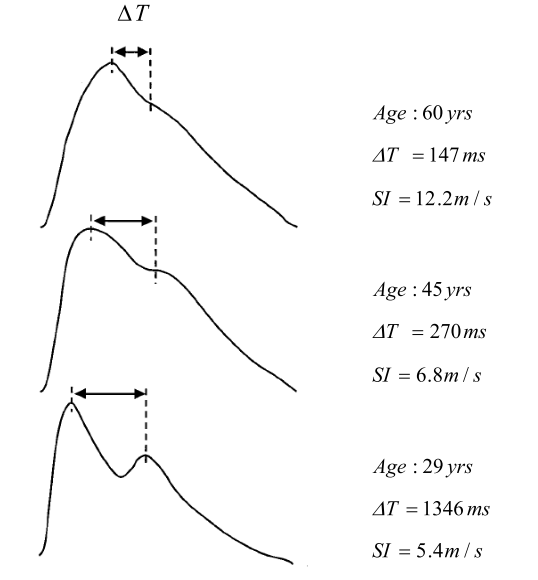
\includegraphics[width=.4\linewidth]{pulse_preprocess/si}
    \caption[SI计算原理示意图]{\label{fig:si}SI计算原理示意图\cite{Elgendi2012,Millasseau2002,Brumfield2005}}
\end{figure}

PWV是指心脏每次搏动射血产生的沿大动脉壁传播的压力波传导速度\cite{Van2012}。在计算PWV时,需要在人体两部位分别测量脉搏波信号。
若记两测量部位的直线距离的80\%为$d$,两部位之间的脉搏波传导时间差为$t$,则有
\begin{equation}
    \label{equ:pwv}
    \text{PWV} = \frac{d}{t}
\end{equation}
PWV已被证实与动脉扩张性、僵硬度、管壁厚度和血液黏稠度密切相关。
特别地,PWV已经在子痫前期的诸多研究中得到应用\cite{Tomsin2012,Katsipi2014,VivianaIvan2018,Ira2014}。
但由于PWV的测量依赖于在人体不同部位测量脉搏波,且测量多利用压力传感器完成,故\textbf{不适用}单点测量的光电容积脉搏波研究。

\section{小结}
本章主要对PPG的信号预处理过程与时域参数描述进行了详细的介绍说明。针对PPG的预处理,对信号滤波、波型检测、重搏波检测、基线漂移去除、重采样及标准化过程进行了介绍,并重点介绍
了一种新型模块化PPG波形检测的SCD算法,该算法具有检测准确度高、抗干扰能力强、可拓展性强等优点。
针对PPG的时域特征参数,从时间类参数、幅度类参数、面积类参数与斜率类参数等方面分别介绍了这些特征参数的定义过程与其可能的生理学意义。
本章的研究内容是后续研究的准备与铺垫。